% !TeX program = xelatex
% !BIB program = biber
%%%%%%%%%%%%%%%%%%%%%%%% TEMPLATE INFO %%%%%%%%%%%%%%%%%%%%%%%%%%%%%%
%:     Template Name = cpe-thesis-th
%:     Version Name  = th-vectier-1.1
%:     Created by:
%:       - Peerapon Siripongwutikorn (peerapon@cpe.kmutt.ac.th), 2016-2020
%:     Modified by:
%:       - Thanin Srithai (thanin.srithai2@mail.kmutt.ac.th), 2021-2022
%:       - Jatetanan Kanchanawat (jate@jate-koh.com), 2024
%:       - Vectier (support@vectier.com), 2024
%:
%: This is a LaTeX template for use in CPE, KMUTT report and thesis.
%%%%%%%%%%%%%%%%%%%%%%%%%%%%%%%%%%%%%%%%%%%%%%%%%%%%%%%%%%%%%%%%%%%%%
%: Instructions:
%: Run at the command line, run: xelatex <filename>.tex
%: Note: Run a few times to generate the output pdf file
%:
%%%%%%%%%%%%%%%%%%%%%%%%%% FILE INFO %%%%%%%%%%%%%%%%%%%%%%%%%%%%%%%%
%:     File name = report.tex
%:     Authors:
%:       - Jatetanan Kanchanawat
%:       - Krid Hepakrone
%:
%%%%%%%%%%%%%%%%%%%%%%%%%%%%%%%%%%%%%%%%%%%%%%%%%%%%%%%%%%%%%%%%%%%%%

%%%%%%%%%%%%%%%%%%%%%%%%%% REPORT START %%%%%%%%%%%%%%%%%%%%%%%%%%%%%
%: NOTE: cpe-thesis-th loads `report`, which only supports 10/11/12pt, so the
%: old `14pt` option was silently ignored. Body size is set below instead.
\documentclass[a4paper,oneside]{cpe-thesis-th}

%%%%%%%%%%%%%%%%%%%%%% Packages and Configs %%%%%%%%%%%%%%%%%%%%%%%%%

\usepackage{color}
\usepackage{pgfgantt}                   % Gantt chart
\usepackage{polyglossia}
\usepackage{caption}                    % Figures and tables captions
\usepackage{pdflscape}                 % Landscape pages for wide diagrams

\usepackage{etoolbox}                   % Patching commands for macros creating i.e. preto
\usepackage{tabularx}
\usepackage{longtable}                  % Long continuous table
\usepackage{ragged2e}                   % Forcing figure
\usepackage{float}                      % ER and checkmark
\usepackage{tikz}                       % Drawing graphs and symbols
\usetikzlibrary{positioning, arrows.meta, fit, backgrounds}
\usepackage{subfig}                     % Subfigures
\usepackage{keyval}                     % Subfigures alignment
\usepackage[export]{adjustbox}          % Subfigures aLignment
\newcommand{\framedgraphic}[2][]{\adjustbox{max width=\linewidth}{\fbox{\includegraphics[#1]{#2}}}}
\usepackage{cleveref}                   % Clever label references
\usepackage{xltabular}   % longtable + tabularx X-columns, breaks across pages

\usepackage{lmodern}
\usepackage{listings}                   % Listings as code blocks
\usepackage{packages/listings-golang}   % Listings support for Golang
\usepackage{packages/listings-yaml}     % Listing support for YAML
\usepackage{packages/report-compat}

%: Biblatex for managing bibliography; instead of using old \bibliography{}
%: NOTE: Biblatex define typesetting onto compilation cache.
%: So recompile from scratch (Remove aux and bbl file and recompile)
%: Everytime you stopped using biblatex

\usepackage[
    backend=biber,      % Biber or Bibtex
    style=ieee,         % Bib standard
    sorting=none,       % Sort by appearance in paper
    % sorting=ynt,       % Sort by year, name...
    % sortcites=true,    % Some other  example options ...
    dateabbrev=true,
    urldate=long,
    block=none,
    indexing=false,
    citereset=none,
    isbn=true,
    url=true,
    doi=true,           % Prints DOI
    natbib=true         % if you need Natbib functions
]{biblatex}

%%%%%%%%%%%%%%%%%% Custom Macros & Settings %%%%%%%%%%%%%%%%%%%%%%%
%: From this part to \begin{document}
%: Do not modify unless you know what you are doing...

%%%%%%%%%%%%%%%%%%%%%%%%%%%%%%%%%
%%%%%%% Biblatex macro %%%%%%%%%%

%: Setup URL access date string
\DefineBibliographyStrings{english}{%
    urlseen = {accessed}
}

%: Reference bib files
%: Make sure you reference correct bib file...
\addbibresource{bib/cyc.bib}
\DeclareLanguageMapping{thai}{english}

%%%%%%%%%%%%%%%%%%%%%%%%%%%%%%%%%
%%%%%%%%% Font settings %%%%%%%%%

%: Define 1st and 2nd language
\setdefaultlanguage{thai}
\setotherlanguage{english}

%: Uncomment following to used Laksaman
%: which is equivalent of Sarabun
% \setmainfont[
%     Scale=1.0,
%     LetterSpace=0,
%     WordSpace=1.0,
%     FakeStretch=1.0,
%     Mapping=tex-text
% ]{Laksaman:script=thai}
% \newfontfamily\thaifont[
%     Scale=1.0,
%     LetterSpace=0,
%     WordSpace=1.0,
%     FakeStretch=1.0,
%     Mapping=tex-text
% ]{Laksaman:script=thai}
% \newfontfamily\thaifonttt{Tlwg Typist:script=thai}

%: Uncomment to use actual Sarabun (font file required)
\newfontfamily\thaifont[Script=Thai,Scale=1.23]{THSarabunNew.ttf}[
    Path=fonts/,
    Extension=.ttf,
    BoldFont=*-Bold,
    ItalicFont=*-Italic,
    BoldItalicFont=*-BoldItalic,
]
\defaultfontfeatures{Mapping=tex-text,Scale=1.23,LetterSpace=0.0}
\setmainfont[Scale=1.23,LetterSpace=0,WordSpace=1.0,FakeStretch=1.0,Mapping=tex-text]{THSarabunNew.ttf}[
    Path=fonts/,
    Extension=.ttf,
    BoldFont=*-Bold,
    ItalicFont=*-Italic,
    BoldItalicFont=*-BoldItalic,
]

%: Set linebreak to Thai
\XeTeXlinebreaklocale "th"
\XeTeXlinebreakskip = 0pt plus 1pt minus 0.1pt
\emergencystretch=3em

%: Define fonts for code blocks
\newfontfamily\codefont[Scale=0.9]{CourierPrime.ttf}[
    Path=fonts/,
    Extension=.ttf,
    BoldFont=*-Bold,
    ItalicFont=*-Italic,
    BoldItalicFont=*-BoldItalic,
]

%%%%%%%%%%%%%%%%%%%%%%%%%%%%%%%%%
%%%%%%%% Margin settings %%%%%%%%
%\linespread{1.6} % Double-spaced
%\oddsidemargin    0.5in
%\evensidemargin   0.5in

%%%%%%%%%%%%%%%%%%%%%%%%%%%%%%%%%
%%%%%%%% Content font size %%%%%%%
%: Body text size in real (rendered) points.
%: TH Sarabun New is loaded with Scale=1.23, so the size LaTeX is asked for
%: is divided by 1.23 to make the rendered size come out at exactly this value.
%: Change \bodyfontsize to resize the whole document (headings follow).
\newdimen\bodyfontsize
\bodyfontsize=16pt

\makeatletter
%: \thsz{\cmd}{size*10}{baseline*10} sets \cmd to a fixed \fontsize. The two numbers
%: are the size10.clo values (in pt) times 10. The numbers are computed once here
%: (not at every use). They are declared robust like the ones in size10.clo, which
%: keeps them safe inside \MakeUppercase (used for chapter headings).
\newcommand\thsz[3]{%
   \begingroup
   \edef\thsz@x{\endgroup\noexpand\DeclareRobustCommand\noexpand#1{\noexpand\@setfontsize\noexpand#1%
      {\strip@pt\dimexpr\bodyfontsize*#2/123\relax}{\strip@pt\dimexpr\bodyfontsize*#3/123\relax}}}%
   \thsz@x}
\thsz\normalsize{100}{120}
\thsz\tiny{50}{60}
\thsz\scriptsize{70}{80}
\thsz\footnotesize{80}{95}
\thsz\small{90}{110}
\thsz\large{120}{140}
\thsz\Large{144}{180}
\thsz\LARGE{173}{220}
\thsz\huge{207}{250}
\thsz\Huge{249}{300}
%: Display math / list spacing that size10.clo attaches to these commands
\g@addto@macro\normalsize{%
   \abovedisplayskip 12\p@ \@plus3\p@ \@minus 6\p@
   \abovedisplayshortskip \z@ \@plus 3\p@
   \belowdisplayshortskip 6.5\p@ \@plus3.5\p@ \@minus 3\p@
   \belowdisplayskip \abovedisplayskip
   \let\@listi\@listI}
\g@addto@macro\footnotesize{%
   \abovedisplayskip 6\p@ \@plus2\p@ \@minus4\p@ \abovedisplayshortskip \z@ \@plus\p@
   \belowdisplayshortskip 3\p@ \@plus\p@ \@minus2\p@ \belowdisplayskip \abovedisplayskip}
\g@addto@macro\small{%
   \abovedisplayskip 8.5\p@ \@plus3\p@ \@minus4\p@ \abovedisplayshortskip \z@ \@plus2\p@
   \belowdisplayshortskip 4\p@ \@plus2\p@ \@minus2\p@ \belowdisplayskip \abovedisplayskip}

%: The class hard-codes heading sizes (12pt / 11pt) for a 10pt body; with a 16pt
%: body they would render smaller than the text. Same layout as cpe-thesis-th.cls,
%: but the sizes keep the class' original ratios to the body (1.2x / 1.1x).
\thsz\thsz@section{120}{168}
\thsz\thsz@subsection{110}{156}
\renewcommand\section{\@startsection{section}{1}{\z@}%
   {-3.5ex \@plus -1ex \@minus -.2ex}{0.1ex\@plus.1ex}%
   {\normalfont\thsz@section\bfseries}}
\renewcommand\subsection{\@startsection{subsection}{2}{\z@}%
   {-3.25ex\@plus -1ex \@minus -.2ex}{0.1ex \@plus .2ex}%
   {\normalfont\thsz@subsection\bfseries}}
\makeatother

%%%%%%%%%%%%%%%%%%%%%%%%%%%%%%%%%
%%%%%% Paragraph Settings %%%%%%%
\linespread{1.15}

\newcommand{\thaijustify}[1]{%
  % \ifnum\value{isfigure}=0
  %   \newline % If counter is set, no newline
  % \fi
  \par\hspace{30pt}\justifying
  #1
  % \vspace{1mm}
  % \setcounter{isfigure}{0}%
}

\newcommand{\thaicaption}[1]{%
  % \ifnum\value{isfigure}=0
  %   \newline % If counter is set, no newline
  % \fi
  \par\justifying
  #1
  % \vspace{1mm}
  % \setcounter{isfigure}{0}%
}

%%%%%%%%%%%%%%%%%%%%%%%%%%%%%%%%%
%%%%%% Caption settings %%%%%%%%%
%: Define how the captions of each report
%: element are formatted.

\captionsetup[table]{
    format=hang,
    labelfont=bf,
    position=top,
    labelsep=space,
    justification=justified,
    singlelinecheck=true
}
\captionsetup[figure]{
    format=hang,
    labelfont=bf,
    position=bottom,
    labelsep=space,
    justification=justified,
    singlelinecheck=true
}
\captionsetup[subfloat]{
    format=hang,
    labelfont=bf,
    labelformat=simple,
    labelsep=period,
    justification=justified,
    singlelinecheck=true
    %listofformat=subparens
}
\captionsetup[lstlisting]{
    format=hang,
    labelfont=bf,
    position=top,
    labelsep=space,
    justification=justified,
    singlelinecheck=true,
    skip=10pt
}
%%%%%%%%%%%%%%%%%%%%%%%%%%%%%%%%%
%%%%%%% Numbering styling %%%%%%%
% Enumerate using arabic numbers
\renewcommand{\labelenumii}{\arabic{enumi}.\arabic{enumii}}
\renewcommand{\labelenumiii}{\arabic{enumi}.\arabic{enumii}.\arabic{enumiii}}
\renewcommand{\labelenumiv}{\arabic{enumi}.\arabic{enumii}.\arabic{enumiii}.\arabic{enumiv}}

%%%%%%%%%%%%%%%%%%%%%%%%%%%%%%%%%
%%%%%% Subfigure settings %%%%%%%

%\renewcommand{\subfigtopskip}{10pt}
%\renewcommand{\subfigbottomskip}{-5pt}
%\renewcommand{\subfigcapskip}{-6pt} %vertical space between caption
%                                    %and figure.
%\renewcommand{\subfigcapmargin}{0pt}

% Use thai alphabets for captions
\renewcommand{\thesubfigure}{\thalph{subfigure}}

%%%%%%%%%%%%%%%%%%%%%%%%%%%%%%%%
%%%%%%% Tikz Settings %%%%%%%%%%
%: Tikz is used for drawing simple edge and node graph
%: Import shapes for usage
\usetikzlibrary{er, positioning, shapes.geometric, arrows}

%: Define checkmark symbol
\def\checkmark{\tikz\fill[scale=0.4](0,.35) -- (.25,0) -- (1,.7) -- (.25,.15) -- cycle;}

%%%%%%%%%%%%%%%%%%%%%%%%%%%%%%%%
%%%%%% Listings Settings %%%%%%%%
%: Listings is used for displaying the program or
%: codes in reports as statement

%: Define text color for code blocks
\definecolor{dkgreen}{rgb}{0,0.6,0}
\definecolor{gray}{rgb}{0.5,0.5,0.5}
\definecolor{mauve}{rgb}{0.58,0,0.82}

%: Define code blocks settings
\lstset{
    frame=tb,
    language=Golang,
    aboveskip=3mm,
    belowskip=3mm,
    showstringspaces=false,
    columns=flexible,
    basicstyle={\small\codefont},
    numbers=left,
    numberstyle=\small\color{gray},
    keywordstyle=\color{blue},
    commentstyle=\color{dkgreen},
    stringstyle=\color{mauve},
    breaklines=false,
    breakatwhitespace=false,
    tabsize=3
}

%%%%%%%%%%%%%%%%%%%%%%%%%%%%%%%%%
%%%%%%%%%% Math macro %%%%%%%%%%%
%: Fraction settings
\renewcommand{\topfraction}{0.85}
\renewcommand{\textfraction}{0.1}

%: Define theorem and proof
\newtheorem{theorem}{Theorem}
\newtheorem{lemma}{Lemma}
\newtheorem{corollary}{Corollary}

%: `proof` and `definition` environments already exist in cpe-thesis-th.cls,
%: so they are intentionally NOT redefined here (a local \def\proof would shadow them).

%\newenvironment{proof}{{\sc Proof:}}{~\hfill \blacksquare}
%% The hyperref package redefines the \appendix. This one
%% is from the dissertation.cls
%\def\appendix#1{\iffirstappendix \appendixcover \firstappendixfalse \fi \chapter{#1}}
%\renewcommand{\arraystretch}{0.8}
%%%%%%%%%%%%%%%%%%%%%%%%%%%%%%%%%

%%%%%%%%%%%%%%%%%%%%% Report Definitions %%%%%%%%%%%%%%%%%%%%%%%%%%
%: Customize below to suit your needs
%: The optional ones can be left blank.

%: First line of title
\def\disstitleone{Your Project Title}
\def\thaidisstitleone{CYC: AI-Driven Platform for UX/UI Development Life Cycle}

%: Second line of title
\def\disstitletwo{}
\def\disstitlethree{}
\def\thaidisstitletwo{}
\def\thaidisstitlethree{}

%: Authors
\def\dissauthorone{}        
\def\thaidissauthorone{นางสาวกัญญ์ญาพัชร ชายทวีป}
\def\dissstudentidone{66070501003}
\def\dissauthortwo{} 
\def\thaidissauthortwo{นายนาวิน แซ่เฮ้ง}
\def\dissstudentidtwo{66070501029}
\def\dissauthorthree{}     
\def\thaidissauthorthree{นายปัณณวิชญ์ หวานแท้}
\def\dissstudentidthree{66070501033}
\def\dissauthorfour{}     
\def\thaidissauthorfour{นายภูบดินทร์ พูลหน่าย}
\def\dissstudentidfour{66070501040}

%: The degree that you're pursuing..
\def\dissdegree{Bachelor of Engineering}        % Name of the degree
\def\thaidissdegree{วิศวกรรมศาสตรบัณฑิต}
\def\dissdegreeabrev{B.Eng}                     % Abbreviation of the degree
\def\dissyear{2026}                             % Year of submission
\def\thaidissyear{2569}                         % Year of submission (B.E.)

%: Advisors
\def\dissadvisor{} % Advisor
\def\thaidissadvisor{ดร.สัณฑวัฒน์ ธัญดิษย์}

%: Note: Leave the following empty if you have no co-advisor
\def\disscoadvisor{} % Co-advisor (optional)
\def\disscoadvisortwo{} % Co-advisor (optional)
\def\thaidisscoadvisor{ผศ.ดร.ปริยกร ปุสวิโร}
\def\thaidisscoadvisortwo{}

%: Committee Members
%: Note: Leave the following empty if no person is in that position
\def\disscommitteetwo{} % 3rd committee member
\def\disscommitteethree{} % 4th committee member (optional)
\def\disscommitteefour{} % 5th committee member (optional)

%: Project Type
\def\worktype{Project}          % Project or Independent study
\def\thaiworktype{ปริญญานิพนธ์}    %  Project or Independent study
\def\disscredit{3}              % 3 credits or 6 credits

%: Department Information
\def\fieldofstudy{Computer Engineering}
\def\department{Computer Engineering}
\def\faculty{Engineering}
\def\thaifieldofstudy{วิศวกรรมคอมพิวเตอร์}
\def\thaidepartment{วิศวกรรมคอมพิวเตอร์}
\def\thaifaculty{วิศวกรรมศาสตร์}

%%%%%%%%%%%%%%%%% Front Page + Signature Page %%%%%%%%%%%%%%%%%%
\begin{document}

% \pdfstringdefDisableCommands{
%   \let\MakeUppercase\relax
% }

% \begin{center}
%   
\includegraphics[width=2.8cm]{./figure/logo02.jpg}
% \end{center}
% \vspace*{-1cm}

% \maketitlepage
% \makesignaturepage

% %%%%%%%%%%%%%%%%%%%%%% English abstract %%%%%%%%%%%%%%%%%%%%%%%%
% \abstract
% [Write your English abstract here.]

% \justifying
% \begin{tabularx}{\textwidth}{@{}l>{\RaggedRight\arraybackslash}X@{}}
%   \textbf{Keywords}: & Keyword1 / Keyword2 / Keyword3
% \end{tabularx}
% \vspace{1mm}
% \endabstract

% %%%%%%%%%%%%%%%%%%%%%%%% Thai abstract %%%%%%%%%%%%%%%%%%%%%%%%%

% \thaiabstract
% \justifying
% [เขียนบทคัดย่อภาษาไทยของคุณที่นี่]

% \justifying
% \begin{tabularx}{\textwidth}{@{}l>{\RaggedRight\arraybackslash}X@{}}
%   & \\
%   \textbf{คำสำคัญ}: & คำสำคัญ1 / คำสำคัญ2 / คำสำคัญ3
% \end{tabularx}
% \vspace{1mm}
% \endabstract

% %%%%%%%%%%%%%%%%%%%%%%%%% Acknowledgments %%%%%%%%%%%%%%%%%%%%%%
% \preface
% [เขียนกิตติกรรมประกาศ/คำขอบคุณของคุณที่นี่]

% %%%%%%%%% Table of Contents, List of Figures/Tables %%%%%%%%%%%%
% %: The three commands below automatically generate the table
% %: of content, list of tables, list of figures, and list of listings

% %: Appendices or Appendix
% %: If you have more than one appendix, use `Appendices`
% \def\appendixnames{Appendices}

% \tableofcontents
% \listoftables
% \listoffigures

% %%%%%%%%%%%%%%%%%%%%%%%% List of codes %%%%%%%%%%%%%%%%%%%%%%%%%
% %: Command below automatically will generate the table
% %: for listing 'lst' package listings

% \listofprograms

%%%%%%%%%%%%%%%%%%%%%%%% List of symbols %%%%%%%%%%%%%%%%%%%%%%%
%: You have to add this manually...

% \listofsymbols
% \newline\justifying{
% \begin{tabular}{@{}p{0.07\textwidth}p{0.7\textwidth}p{0.1\textwidth}}
% \textbf{สัญลักษณ์} & & \textbf{หน่วย} \\[0.2cm]
%     $\alpha$ & Test variable\hfill & m$^2$ \\
%     $\lambda$ & Interarival rate\hfill &  jobs/second\\
%     $\mu$ & Service rate\hfill & jobs/second\\
% \end{tabular}
% }

%\setlength{\parskip}{1.2mm}

\newgeometry{left=2.5cm,right=2.5cm,top=2.5cm,bottom=2.5cm}
\begin{titlepage}
  \thispagestyle{empty}
  \setlength{\parindent}{0pt}
  \setlength{\parskip}{0pt}
  \fontsize{14}{18}\selectfont

  \begin{center}
    \textbf{ข้อเสนอโครงงานวิศวกรรมคอมพิวเตอร์}\\[4pt]
    \textbf{หลักสูตรวิศวกรรมศาสตรบัณฑิต สาขาวิชาวิศวกรรมคอมพิวเตอร์}\\[4pt]
    \textbf{ปีการศึกษา 2569}
  \end{center}
  \vspace{9mm}

  \textbf{หัวข้อโครงงาน} \thaidisstitleone
  \vspace{5mm}

  \textbf{สมาชิกกลุ่ม}\par
  \begingroup
    \fontsize{14}{18}\selectfont
    \setlength{\tabcolsep}{3pt}
    \renewcommand{\arraystretch}{1}
    \begin{tabularx}{\textwidth}{@{}r>{\RaggedRight\arraybackslash}Xl@{}}
      \hspace*{12mm}\dissstudentidone & \thaidissauthorone \\
      \dissstudentidtwo & \thaidissauthortwo \\
      \dissstudentidthree & \thaidissauthorthree \\
      \dissstudentidfour & \thaidissauthorfour \\
    \end{tabularx}
  \endgroup
  \par\vspace{5mm}

  \textbf{อาจารย์ที่ปรึกษา}\par
  \hspace*{12mm} \thaidissadvisor\par
  \vspace{5mm}

  \textbf{อาจารย์ที่ปรึกษาร่วม}\par
  \hspace*{12mm} \thaidisscoadvisor\par

  \vspace{48mm}

  \fontsize{13}{16}\selectfont By signing this, I hereby acknowledge that I have read the proposal and approved this Project\par
  \vspace{32mm}

  \begin{tabular*}{\textwidth}{@{\extracolsep{\fill}}>{\centering\arraybackslash}p{0.45\textwidth}>{\centering\arraybackslash}p{0.45\textwidth}@{}}
  & \hrulefill \\
  & \thaidissadvisor \\
  & อาจารย์ที่ปรึกษา \\
\end{tabular*}



  
\end{titlepage}

%%%%%%%%%%%%%%%%%%%%% List of vocabs & terms %%%%%%%%%%%%%%%%%%%
%: Add your own terms and definitions below, following the example format.
\newcommand{\tableraglf}[1]{\RaggedRight{#1}}
\listofvocab
\begin{flushleft}
  \begin{xltabular}{\textwidth}{@{}>{\RaggedRight\arraybackslash}p{0.31\textwidth}@{\quad=\quad}>{\RaggedRight\arraybackslash}X@{}}
     UX/UI Design / การออกแบบประสบการณ์ผู้ใช้และส่วนต่อประสานผู้ใช้ & \tableraglf{กระบวนการออกแบบที่ครอบคลุมสองส่วนหลัก คือ UX (User Experience) ซึ่งเน้นการออกแบบภาพรวมของประสบการณ์ที่ผู้ใช้ได้รับขณะใช้งานผลิตภัณฑ์หรือบริการ เช่น ความง่ายในการใช้งาน ความสะดวก และความพึงพอใจ และ UI (User Interface) ซึ่งเน้นการออกแบบส่วนต่อประสานที่ผู้ใช้มองเห็นและโต้ตอบด้วยโดยตรง เช่น ปุ่มกด เมนู สี และรูปแบบตัวอักษร โดยทั้งสองส่วนทำงานร่วมกันเพื่อให้ผลิตภัณฑ์ดิจิทัล เช่น เว็บไซต์หรือแอปพลิเคชัน ใช้งานได้ง่าย มีประสิทธิภาพ และตอบสนองความต้องการของผู้ใช้ได้อย่างแท้จริง} \\

    UX/UI development life cycle (UX/UI DLC) & \tableraglf{วงจรการพัฒนางานออกแบบ UX/UI ซึ่งเป็นกระบวนการที่มีขั้นตอนต่อเนื่องกันตั้งแต่การเริ่มต้นจนถึงการนำไปใช้งานจริง โดยทั่วไปประกอบด้วยขั้นตอนหลัก เช่น การวิจัยและทำความเข้าใจผู้ใช้ (Research) การกำหนดปัญหาและความต้องการ (Define) การออกแบบแนวคิดและโครงร่าง (Ideate) การสร้างต้นแบบ (Prototype) และการทดสอบกับผู้ใช้จริง (Testing) ทั้งนี้ในแต่ละรอบของวงจรมักมีการนำผลตอบรับกลับมาปรับปรุงซ้ำ (Iteration) เพื่อให้ผลิตภัณฑ์ตอบโจทย์ผู้ใช้ได้ดียิ่งขึ้น} \\
    
    A/B Testing & \tableraglf{วิธีการทดสอบการใช้งานกับผู้เข้าร่วมทดสอบ โดยให้ผู้เข้าร่วมทดสอบทดลองใช้งานต้นแบบผลิตภัณฑ์สองรูปแบบที่มีเป้าประสงค์เดียวกันเพื่อเปรียบเทียบประสิทธิภาพการใช้งานและให้ข้อคิดเห็นหรือข้อเสนอแนะเกี่ยวกับรูปแบบหรือผลิตภัณฑ์นั้น ๆ พร้อมทั้งเลือกรูปแบบใดรูปแบบหนึ่งที่เห็นว่าเหมาะสมกับเป้าประสงค์นั้น ๆ} \\
    
    Usability Testing / การทดสอบการใช้งาน & \tableraglf{กระบวนการทดสอบการใช้งาน โดยให้ผู้เข้าร่วมทดสอบลองใช้งานระบบและหาจุดที่ใช้งานยากหรือติดขัด ซึ่งในขณะที่ทำการทดสอบ ผู้เข้าร่วมการทดสอบจำเป็นต้องคิดไปด้วยพูดไปด้วย (Thinking-Aloud) โดยนักออกแบบจะคอยสังเกตพฤติกรรมการใช้งานและรับฟังความเห็นของผู้เข้าร่วมทดสอบขณะทำภารกิจที่กำหนด} \\

    Contextual Feedback / ข้อเสนอแนะเชิงบริบท & \tableraglf{ข้อคิดเห็นหรือคำแนะนำที่กล่าวเฉพาะเจาะจงกับสิ่งใดสิ่งหนึ่ง เพื่อให้คำแนะนำมีความเกี่ยวข้องและนำไปใช้ได้ตรงจุดมากขึ้น} \\

    Wireframe / โครงร่างหน้าจอ & \tableraglf{โครงร่างพื้นฐานแสดงตำแหน่งองค์ประกอบบนหน้าจอ โดยยังไม่เน้นสีสันหรือรายละเอียดด้านภาพ ใช้สื่อสารการจัดวางในขั้นต้นของการออกแบบ} \\

    Prototype / ต้นแบบ & \tableraglf{ต้นแบบผลิตภัณฑ์ที่สร้างขึ้นเพื่อทดสอบแนวคิดก่อนพัฒนาจริง สามารถโต้ตอบได้ในระดับหนึ่ง แบ่งเป็นสามระดับตามความน้อย-มากของรายละเอียดในต้นแบบ คือ low, mid, high-fidelity prototype} \\

    Design System & \tableraglf{ชุดมาตรฐานการออกแบบที่รวบรวมองค์ประกอบ กฎเกณฑ์ และแนวทางปฏิบัติไว้ในที่เดียว เช่น สี ตัวอักษร ไอคอน และ component ต่าง ๆ เพื่อให้การออกแบบผลิตภัณฑ์มีความสอดคล้องและเป็นมาตรฐานเดียวกันทั้งระบบ} \\

    Insight / ข้อมูลเชิงลึก & \tableraglf{ความเข้าใจที่ได้จากการวิเคราะห์ข้อมูลหรือพฤติกรรมผู้ใช้ ซึ่งเปิดเผยปัญหาหรือความต้องการที่ซ่อนอยู่} \\

    User / ผู้ใช้ & \tableraglf{บุคคลที่มีปฏิสัมพันธ์โดยตรงกับผลิตภัณฑ์ ระบบ หรือบริการ เพื่อบรรลุเป้าหมายของตนเอง} \\

    Generative AI & \tableraglf{เทคโนโลยีปัญญาประดิษฐ์ที่สามารถสร้างเนื้อหาใหม่ เช่น ข้อความ ภาพ เสียง หรือโค้ดจากคำสั่ง (prompt)} \\

    Design Intent & \tableraglf{เจตนาหรือเป้าหมายเชิงการออกแบบที่นักออกแบบต้องการสื่อสาร ใช้เป็นแนวทางตัดสินใจในการออกแบบ} \\

    Component & \tableraglf{ส่วนประกอบย่อยที่นำกลับมาใช้ซ้ำได้ใน UI เช่น ปุ่มหรือช่องกรอกข้อมูล ช่วยให้การออกแบบสอดคล้องกัน} \\

    Multi-variant UI & \tableraglf{UI ที่มีสองรูปแบบ} \\

    Human-in-the-loop & \tableraglf{แนวคิดที่มนุษย์เข้ามาใช้วิจารณญาณตรวจสอบและปรับปรุงผลลัพธ์จากปัญญาประดิษฐ์แบบรู้สร้าง เพื่อความถูกต้องเหมาะสม} \\

    Stakeholder / ผู้มีส่วนได้เสีย & \tableraglf{บุคคลหรือกลุ่มที่มีส่วนได้ส่วนเสียกับโครงการ เช่น ผู้บริหารหรือผู้ว่าจ้าง ซึ่งมีบทบาทในการตัดสินใจหรือสนับสนุนโครงการ} \\

    Cognitive Overload & \tableraglf{ภาวะที่ได้รับข้อมูลมากเกินความสามารถในการประมวลผลของสมอง ส่งผลให้สับสนหรือตัดสินใจผิดพลาด} \\

    Requirement / ความต้องการ & \tableraglf{เงื่อนไขที่ผลิตภัณฑ์ต้องมีเพื่อตอบสนองความต้องการผู้ใช้หรือเป้าประสงค์ของโครงการ} \\

    Usability Tester / ผู้เข้าร่วมทดสอบ & \tableraglf{บุคคลที่เข้าร่วมทดสอบการใช้งานผลิตภัณฑ์ พร้อมให้ข้อคิดเห็นเพื่อนำไปปรับปรุงการออกแบบ} \\

    Persona Artifact & \tableraglf{เอกสารจำลองลักษณะผู้ใช้กลุ่มเป้าหมาย เช่น ชื่อ อายุ พฤติกรรม และเป้าหมาย เพื่อให้ทีมออกแบบเข้าใจผู้ใช้ชัดเจนขึ้น} \\
    %  & \tableraglf{ } \\
    
    %  & \tableraglf{ } \\
    
    %  & \tableraglf{ } \\
    
    %  & \tableraglf{ } \\
    
    %  & \tableraglf{ } \\
  \end{xltabular}
\end{flushleft}

\restoregeometry

%%%%%%%%%%%%%%%%%%%%%%% Main body %%%%%%%%%%%%%%%%%%%%%%%%%%%%%%

\chapter{บทนำ}
% \thaijustify{
%   [ภาพรวมของบทนี้]
% }
\section{ที่มาและความสำคัญ}
\thaijustify{
  การออกแบบประสบการณ์ผู้ใช้และส่วนต่อประสานผู้ใช้ (UX/UI Design) โดยปกติมีลักษณะเป็นกระบวนการที่วนซ้ำและยึดผู้ใช้เป็นศูนย์กลาง ทว่าในทางปฏิบัตินักออกแบบมักถูกจำกัดด้วยเวลา ประสบการณ์ และทรัพยากร กระบวนการออกแบบเริ่มตั้งแต่การรับโจทย์ รวบรวมความต้องการ ทำความเข้าใจผู้ใช้ นิยามปัญหา ระดมความคิด สร้างต้นแบบ และทดสอบ ในขณะเดียวกันยังต้องทำงานร่วมกับนักพัฒนาซอฟต์แวร์และผู้มีส่วนได้ส่วนเสีย ในกระบวนการสร้าง wireframe และ prototype มักถูกสร้างขึ้นด้วยมือ กระบวนการนี้จึงใช้แรงงานและเวลามาก จนมักไม่เหลือเวลาสำหรับการทดสอบการใช้งานกับผู้ใช้จริงก่อนส่งมอบงาน ด้วยเหตุนี้ ทีมผู้พัฒนาจึงมักทดสอบกับผู้เข้าร่วมทดสอบไม่มากพอที่จะเห็นปัญหาและแก้ไขได้ทันก่อนกำหนดการส่งมอบ \cite{suh2025storyensemble} สิ่งนี้ก่อให้เกิดช่องว่างระหว่างผลิตภัณฑ์ที่ส่งมอบกับความต้องการที่แท้จริงของผู้ใช้ ซึ่งเป็นผลมาจากการตัดสินใจเชิงออกแบบที่ถูกกำหนดโดยแรงกดดันด้านเวลามากกว่า insight จากผู้ใช้จริง}

\thaijustify{
  งานวิจัยที่ผ่านมาชี้ว่า Generative AI สามารถช่วยลดภาระทางด้านเวลาและแรงงานในการสร้าง prototype และลดปัญหาคอขวดของการทดสอบได้ อย่างไรก็ตาม เครื่องมือที่มีอยู่ในปัจจุบันยังคงกระจัดกระจายและส่วนใหญ่มุ่งเน้นเฉพาะงานใดงานหนึ่งเป็นหลัก ยังไม่ถูกนำมาใช้ตลอดทั้ง UX/UI Development Life Cycle \cite{chung2025ureka, lu2022bridging}
}

% \thaijustify{
%   งานวิจัยที่ผ่านมาชี้ให้เห็นว่า Generative AI สามารถช่วยลดช่องว่างดังกล่าวได้ โดยทำให้แต่ละรอบของการวนซ้ำใช้เวลาน้อยลงและส่งผลให้มีการวนซ้ำอย่างสม่ำเสมอในกระบวนการพัฒนาผลิตภัญฑ์เป็นไปได้ในทางปฏิบัติ ผลการศึกษาแสดงให้เห็นว่า Generative AI สามารถสร้าง wireframe ได้โดยอัตโนมัติจากการอธิบาย design intent ด้วยภาษาธรรมชาติ \cite{feng2023designing} และยังสามารถสร้าง high-fidelity prototype ได้ทั้งระดับภาพรวมทั้งระบบและระดับ component \cite{yuan2024towards} ซึ่งช่วยลดต้นทุนด้านเวลาและแรงงานของการออกแบบในแต่ละรอบ นอกจากการทำให้การวนซ้ำทดสอบเกิดบ่อยขึ้นแล้ว สภาพแวดล้อมการออกแบบแบบ forward-backward propagation ยังเปิดโอกาสให้ทีมผู้พัฒนาย้อนกลับไปทบทวนและปรับแก้การตัดสินใจก่อนหน้าได้อย่างเป็นพลวัตตลอดหลายรอบการทำงาน แทนที่จะดำเนินไปข้างหน้าเพียงอย่างเดียว \cite{suh2025storyensemble} แนวทางนี้สอดคล้องกับงานวิจัยด้านการใช้งาน (usability) ที่เป็นที่ยอมรับ ซึ่งแสดงให้เห็นว่าการทดสอบบ่อยครั้งด้วยกลุ่มตัวอย่างขนาดเล็กให้ insight ที่นำไปปรับใช้ได้จริงมากกว่าการทดสอบขนาดใหญ่ที่ทำน้อยครั้งกว่า \cite{nielsen2000five} เมื่อพิจารณาโดยรวม งานวิจัยเหล่านี้ชี้ว่า Generative AI สามารถช่วยลดภาระทางด้านเวลาและแรงงานในการสร้าง prototype และปัญหาคอขวดของการทดสอบได้ อย่างไรก็ตาม เครื่องมือที่มีอยู่ในปัจจุบันยังคงกระจัดกระจายและส่วนใหญ่มุ่งเน้นเฉพาะงานใดงานหนึ่งเป็นหลัก ยังไม่ถูกนำมาใช้ตลอดทั้ง UX/UI DLC \cite{chung2025ureka, lu2022bridging}}

\thaijustify{
  เพื่อเพิ่มประสิทธิภาพ UX/UI DLC โครงงานนี้ให้ความสำคัญกับกระบวนการ A/B testing เป็นพิเศษ ซึ่งการทำ A/B testing ซ้ำหลายรอบ นักออกแบบจำเป็นต้องจัดเตรียม multi-variant UI, รวบรวมและจัดระเบียบข้อเสนอแนะจากผู้ใช้, ตลอดจนตีความผลลัพธ์ที่ได้ก่อนเริ่มการวนซ้ำรอบถัดไปด้วยตนเอง เพื่อสนับสนุนกระบวนการดังกล่าว ผู้พัฒนาจึงนำเสนอแพลตฟอร์มที่บูรณาการปัญญาประดิษฐ์แบบรู้สร้างที่มีอยู่เข้ากับกระบวนการ A/B testing กล่าวคือ นักออกแบบสามารถอธิบาย design intent จากนั้นแพลตฟอร์มจะสร้าง multi-variant UI สำหรับทำ A/B testing และผู้เข้าร่วมทดสอบสามารถให้ข้อเสนอแนะเชิงบริบทด้วยการเลือก component ที่ต้องการให้ข้อเสนอแนะ และข้อเสนอแนะเหล่านี้จะถูกนำไปรวบรวม กลั่นกรอง โดยปัญญาประดิษฐ์ร่วมกับนักออกแบบเพื่อสร้าง multi-variant UI ใหม่สำหรับการทำ A/B testing ในรอบถัดไป}

\thaijustify{
  นอกจากนี้ แพลตฟอร์มดังกล่าวยังมุ่งสร้างขั้นตอนการทำงานร่วมกันระหว่างมนุษย์และปัญญาประดิษฐ์อย่างสมดุล (human-in-the-loop) โดยในขั้นแรกปัญญาประดิษฐ์จะสรุปและวิเคราะห์ข้อเสนอแนะที่ได้รับจากรอบการทดสอบ เพื่อระบุรูปแบบ ข้อมูลเชิงลึก และประเด็นสำคัญ ในขั้นนี้ นักออกแบบจะเข้ามามีบทบาทในการพิจารณาผลการวิเคราะห์ที่ปัญญาประดิษฐ์สร้างขึ้น ใช้การตัดสินใจอย่างมืออาชีพและมีวิจารณญาณในการกำหนดทิศทางการออกแบบ \cite{chung2025ureka} เมื่อนักออกแบบตรวจสอบและยืนยันแนวทางแล้ว ปัญญาประดิษฐ์แบบรู้สร้างจะดำเนินการตามที่นักออกแบบกำหนดเพื่อสร้าง multi-variant UI สำหรับรอบการทดสอบถัดไป อีกทั้งยังสร้างรายงานการออกแบบ ที่บันทึกว่าได้รับข้อเสนอแนะใดบ้าง ข้อเสนอแนะนั้นได้รับการตีความโดยปัญญาประดิษฐ์และนักออกแบบตัดสินใจอย่างไร เพื่อเป็นเหตุผลประกอบที่ชัดเจนและมีข้อมูลสนับสนุนสำหรับการสื่อสารกับผู้มีส่วนได้ส่วนเสีย โดยสรุป โครงงานนี้มีเป้าหมายเพื่อแสดงให้เห็นว่าแพลตฟอร์มที่เสริมศักยภาพด้วยการใช้ปัญญาประดิษฐ์ร่วมกับมนุษย์ใน UX/UI DLC สามารถลดระยะเวลาและภาระงานที่ต้องทำด้วยมือ เพิ่มความถี่ของวงรอบการทดสอบ และยกระดับคุณภาพโดยรวมตลอดจนเป็นเครื่องมือที้ใช้ตรวจสอบย้อนกลับการตัดสินใจตลอดทั้งกระบวนการได้}


\section{วัตถุประสงค์}
\thaijustify{
  \begin{enumerate}

    \item เพื่อให้นักออกแบบสามารถอธิบายว่าข้อเสนอแนะจากผู้ใช้ส่งผลต่อการตัดสินใจเชิงออกแบบอย่างไร และสามารถนำเหตุผลประกอบที่สืบกลับได้ไปใช้สร้าง persona สำหรับผู้มีส่วนได้ส่วนเสียแต่ละกลุ่ม เพื่อใช้เป็นเหตุผลรองรับโดยมีข้อมูลสนับสนุนผลลัพธ์การออกแบบในขั้นสุดท้าย

    \item เพื่อลดภาระงานที่ต้องทำด้วยมือและระยะเวลาที่นักออกแบบต้องใช้ในการสร้าง multi-variant UI prototype สำหรับ A/B testing

    \item เพื่อเสริมศักยภาพให้นักออกแบบสามารถดำเนินการทดสอบกับผู้ใช้ได้บ่อยครั้งและสม่ำเสมอภายใต้กรอบเวลาส่งมอบงานที่จำกัด โดยอาศัยปัญญาประดิษฐ์แบบรู้สร้างในการปรับปรุงการออกแบบบนพื้นฐานของข้อเสนอแนะที่ผ่านการตรวจสอบยืนยันแล้ว และนำไปทำ A/B testing ในรอบถัดไป

    \item เพื่อให้ผู้เข้าร่วมทดสอบ A/B testing สามารถให้ข้อเสนอแนะเชิงบริบทมากขึ้นและใช้ความพยายามน้อยลง

    \item เพื่อลด effort ของนักออกแบบในการวิเคราะห์ข้อเสนอแนะจากผู้ใช้ที่มีปริมาณมาก
\end{enumerate}
}
\section{ขอบเขต}
\thaijustify{
  \begin{enumerate}
    \item ใช้โมเดล Generative AI ที่มีอยู่ในปัจจุบันเพื่อสร้าง multi-variant UI prototype จากการอธิบายความต้องการทางการออกแบบด้วยภาษาธรรมชาติ
    \item จัดเตรียมสภาพแวดล้อมสำหรับให้ผู้เข้าร่วมทดสอบ A/B testing ตรวจสอบ เปรียบเทียบ และให้ข้อเสนอแนะเชิงบริบท
    \item ใช้แบบโมเดลปัญญาประดิษฐ์ที่มีอยู่ในปัจจุบันในการรวบรวมข้อเสนอแนะและระบุรูปแบบ ข้อมูลเชิงลึก และประเด็นสำคัญเพื่อพิจารณา โดยยังคงให้นักออกแบบเป็นผู้ตัดสินใจ (human-in-the-loop) ก่อนเริ่มการทำ A/B testing ในรอบถัดไป
    \item ใช้การวิเคราะห์ที่ได้จากปัญญาประดิษฐ์ในการเชื่อมโยงข้อเสนอแนะของผู้ใช้เข้ากับวิวัฒนาการของการออกแบบและสร้างรายงาน
  \end{enumerate}
}
\section{แผนการดำเนินงาน}
\subsection{การแบ่งงานย่อย}
\begin{enumerate}
  \item \textbf{การจัดทำเอกสาร}
    \begin{itemize}
      \item การเลือกหัวข้อโครงงาน
      \item เอกสารแนวคิดโครงงาน
      \item การทบทวนวรรณกรรม
      \item รายงานข้อเสนอโครงงาน
      \item การนำเสนอข้อเสนอโครงงาน
      \item รายงานความก้าวหน้าภาคเรียนที่ 1
      \item การนำเสนอผลงานภาคเรียนที่ 1
      \item รายงานฉบับสมบูรณ์
      \item การนำเสนอโครงงานฉบับสมบูรณ์
    \end{itemize}

  \item \textbf{การวิเคราะห์ Requirements และการออกแบบระบบ}
    \begin{itemize}
      \item การสัมภาษณ์ผู้มีส่วนได้ส่วนเสีย
      \item การวิเคราะห์ Requirements
      \item Functional และ Non-Functional Requirements
      \item Use Cases และ Sequence Diagram
      \item System Architecture
      \item AI Workflow และ Prompt Architecture
      \item การออกแบบฐานข้อมูล
      \item การออกแบบ API
      \item การออกแบบ UI/UX (User Flow และ Wireframe)
      \item Prototype ของระบบ
    \end{itemize}

  \item \textbf{M0: พื้นฐาน}
    \begin{itemize}
      \item ยืนยัน personas, ขอบเขตงาน และ MVP
      \item กำหนด data model (org, project, story, variant, session, task, feedback, round, report)
      \item เลือก architecture: auth, LLM provider, prototype rendering, hosting
      \item สำรวจและเลือก design system และ UI kit
      \item กำหนด requirements ด้าน PDPA และข้อความขอ consent
      \item ตั้งค่า CI/CD, environments และ event analytics
      \item กำหนด sprint plan
    \end{itemize}

  \item \textbf{M1: การเข้าถึงระบบอย่างปลอดภัย}
    \begin{itemize}
      \item Homepage และ entry points
      \item หน้า Register พร้อม validation (อีเมลนี้ถูกลงทะเบียนแล้ว, อีเมล/รหัสผ่านไม่ตรงตามกฎ, ลองใหม่)
      \item การยืนยันอีเมลแบบ non-blocking
      \item Sign-in พร้อม error handling (credentials ไม่ถูกต้อง, ลองใหม่)
      \item Forgot password: ส่งคำขอ, อีเมลสำหรับ reset, link หมดอายุ, ส่งคำขออีกครั้ง, reset สำเร็จ
      \item Role และ permission engine
      \item Role-based routing (Designer, Client, Developer, PM) ส่วน Tester เข้าผ่าน session
      \item Auth QA และการทดสอบ access control
    \end{itemize}

  \item \textbf{M2: การตั้งค่า Project}
    \begin{itemize}
      \item ตรวจสอบ organization ที่มีอยู่เดิม จากนั้นสร้างหรือเลือก org / project hub
      \item สร้าง project
      \item ฟอร์ม design intent: คำอธิบาย, persona, guideline, brand color/CI/tone of voice
      \item จัดเก็บ design intent เป็น AI context ที่นำกลับมาใช้ซ้ำได้
    \end{itemize}

  \item \textbf{M3: การสร้างงานออกแบบด้วย AI}
    \begin{itemize}
      \item สร้าง user story และ problem statement
      \item Prompt builder ที่ผสาน design intent เข้ากับ story
      \item การสร้าง UI หลาย variant (LLM integration, guardrails, สถานะ loading และ failure)
      \item การปรับแต่ง UI ผ่าน chat
      \item การ preview variant และการ render interactive prototype
      \item Approve และ assign ให้ tester: tasks และคำถาม feedback
      \item เริ่ม testing session: สร้าง code/link
      \item Evaluation set สำหรับประเมินคุณภาพ output ของ AI
    \end{itemize}

  \item \textbf{M4: Testing Space}
    \begin{itemize}
      \item การเข้า session ด้วย code หรือ link พร้อมตรวจสอบความถูกต้อง
      \item End states: session ถูกปิด/ไม่ถูกต้อง และกรณีที่ submit ไปแล้ว
      \item PDPA consent พร้อม logging และหากปฏิเสธจะออกจาก session โดยไม่มีการเก็บข้อมูลใด ๆ
      \item Assign ผู้ใช้ให้กับ test
      \item Onboarding สำหรับเครื่องมือทดสอบ
      \item Task runner พร้อม interaction capture
      \item Walkthrough หลังทำ task และคำถามแบบเจาะจง
      \item Commenting: annotate ที่ component, comment ทั้งหน้า, skip
      \item Loop สำหรับ task ที่เหลือ และการจบการทดสอบของ tester
      \item การทดสอบ cross-browser
    \end{itemize}

  \item \textbf{M5: Feedback}
    \begin{itemize}
      \item Session monitoring (รอ tester)
      \item การรวบรวมและ aggregate feedback
      \item การวิเคราะห์ด้วย AI: themes, tagging และสรุปผล
      \item Designer review UI: retag, merge, split, notes, mark "not fixing" พร้อมระบุเหตุผล
      \item Loop การ approve หรือ revise
      \item นำ feedback ที่เลือกไปใส่ใน prompt ของ round ถัดไป
      \item การตัดสินใจจบ session, round versioning และ history
      \item การทดสอบ loop แบบ end-to-end
    \end{itemize}

  \item \textbf{M6: รายงานสำหรับ Stakeholder}
    \begin{itemize}
      \item รายการ project (read-only, เฉพาะ round ที่ approve แล้ว)
      \item Client view: acknowledge และ comment โดยแยกจาก feedback ของ tester
      \item Developer handoff: export spec/code และ technical risks ที่ถูก flag ไว้
      \item PM status: ความคืบหน้าของ round และ timeline gap
      \item Report generation engine (เป้าหมายทางธุรกิจ, tester artifact, feedback, design decision, component/code, งบประมาณ/timeline)
      \item จัดทำรายงานแยกตาม role ทั้ง 3 ฉบับให้เสร็จสมบูรณ์
      \item การ export และแชร์รายงาน (PDF หรือ link)
    \end{itemize}

  \item \textbf{M7: Pilot และ Launch}
    \begin{itemize}
      \item การทดสอบ regression ทั้งระบบ และ UAT
      \item Security review และ PDPA audit
      \item Load test กับ tester ที่ใช้งานพร้อมกัน
      \item Pilot กับทีมจริง 2--3 ทีม และเก็บ feedback
      \item Help docs, onboarding และกระบวนการ support
      \item Monitoring และ business KPI dashboard
      \item Go-live และ retrospective
    \end{itemize}
\end{enumerate}

\subsection{Gantt chart}
\begin{figure}[H]
  \centering
  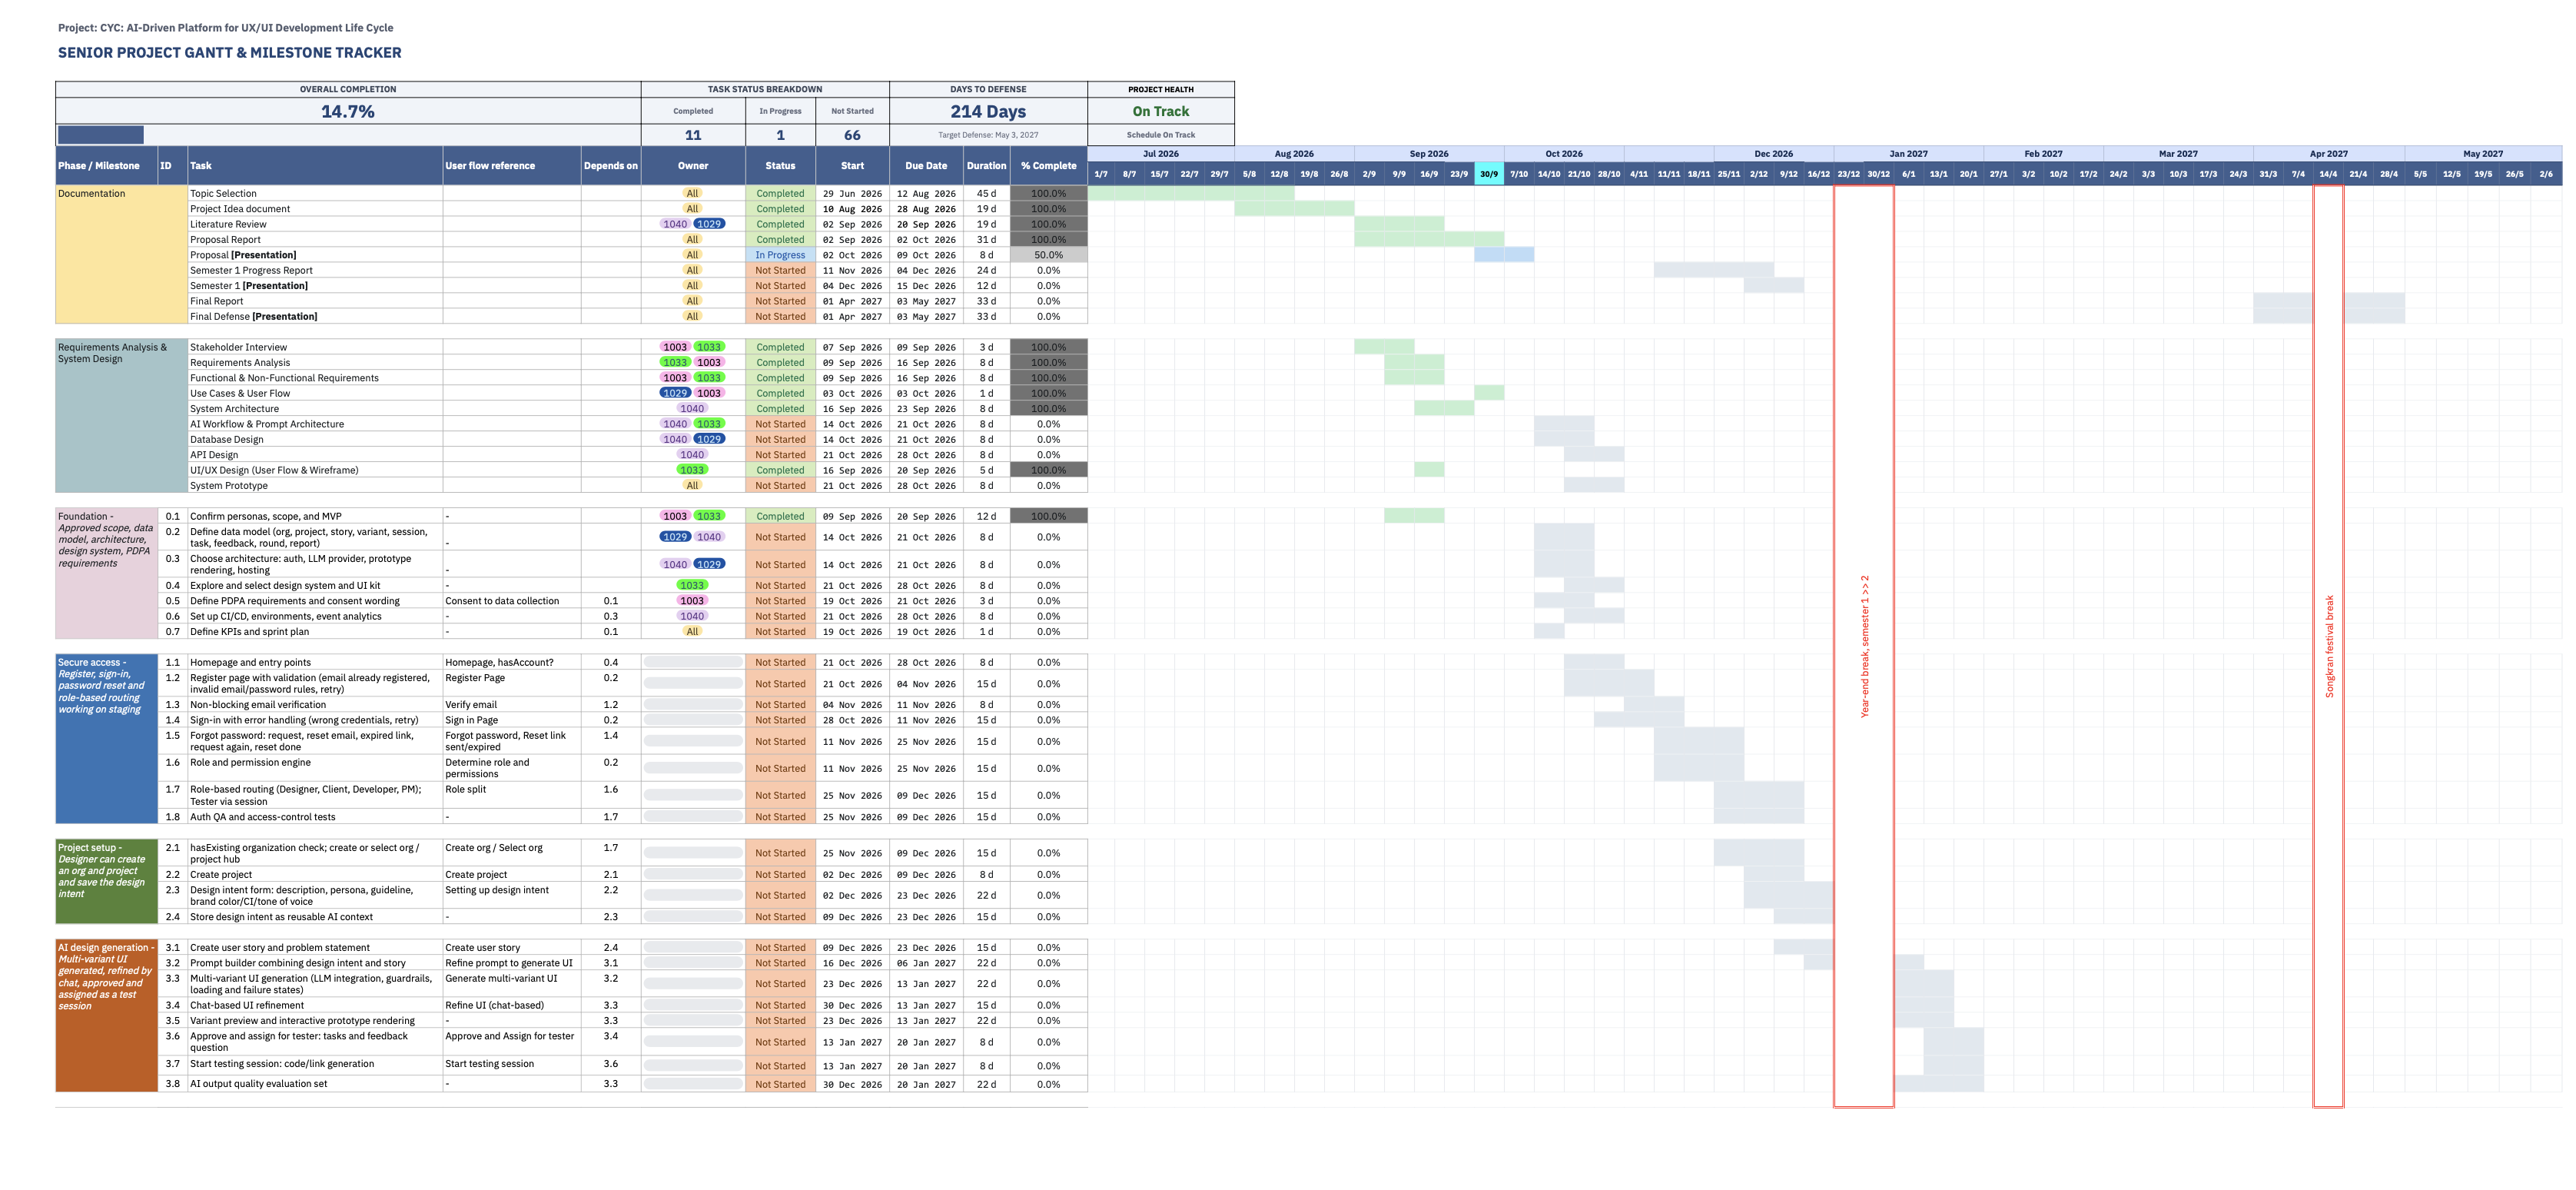
\includegraphics[
    width=0.9\textheight,
    height=0.95\linewidth,
    keepaspectratio,
    angle=90,
    origin=c
  ]{figure/gantt-sem1.png}
  \caption{Project Gantt chart สำหรับภาคการศึกษาที่ 1}
  \label{fig:gantt-semester-1}
\end{figure}

\clearpage

\begin{figure}[H]
  \centering
  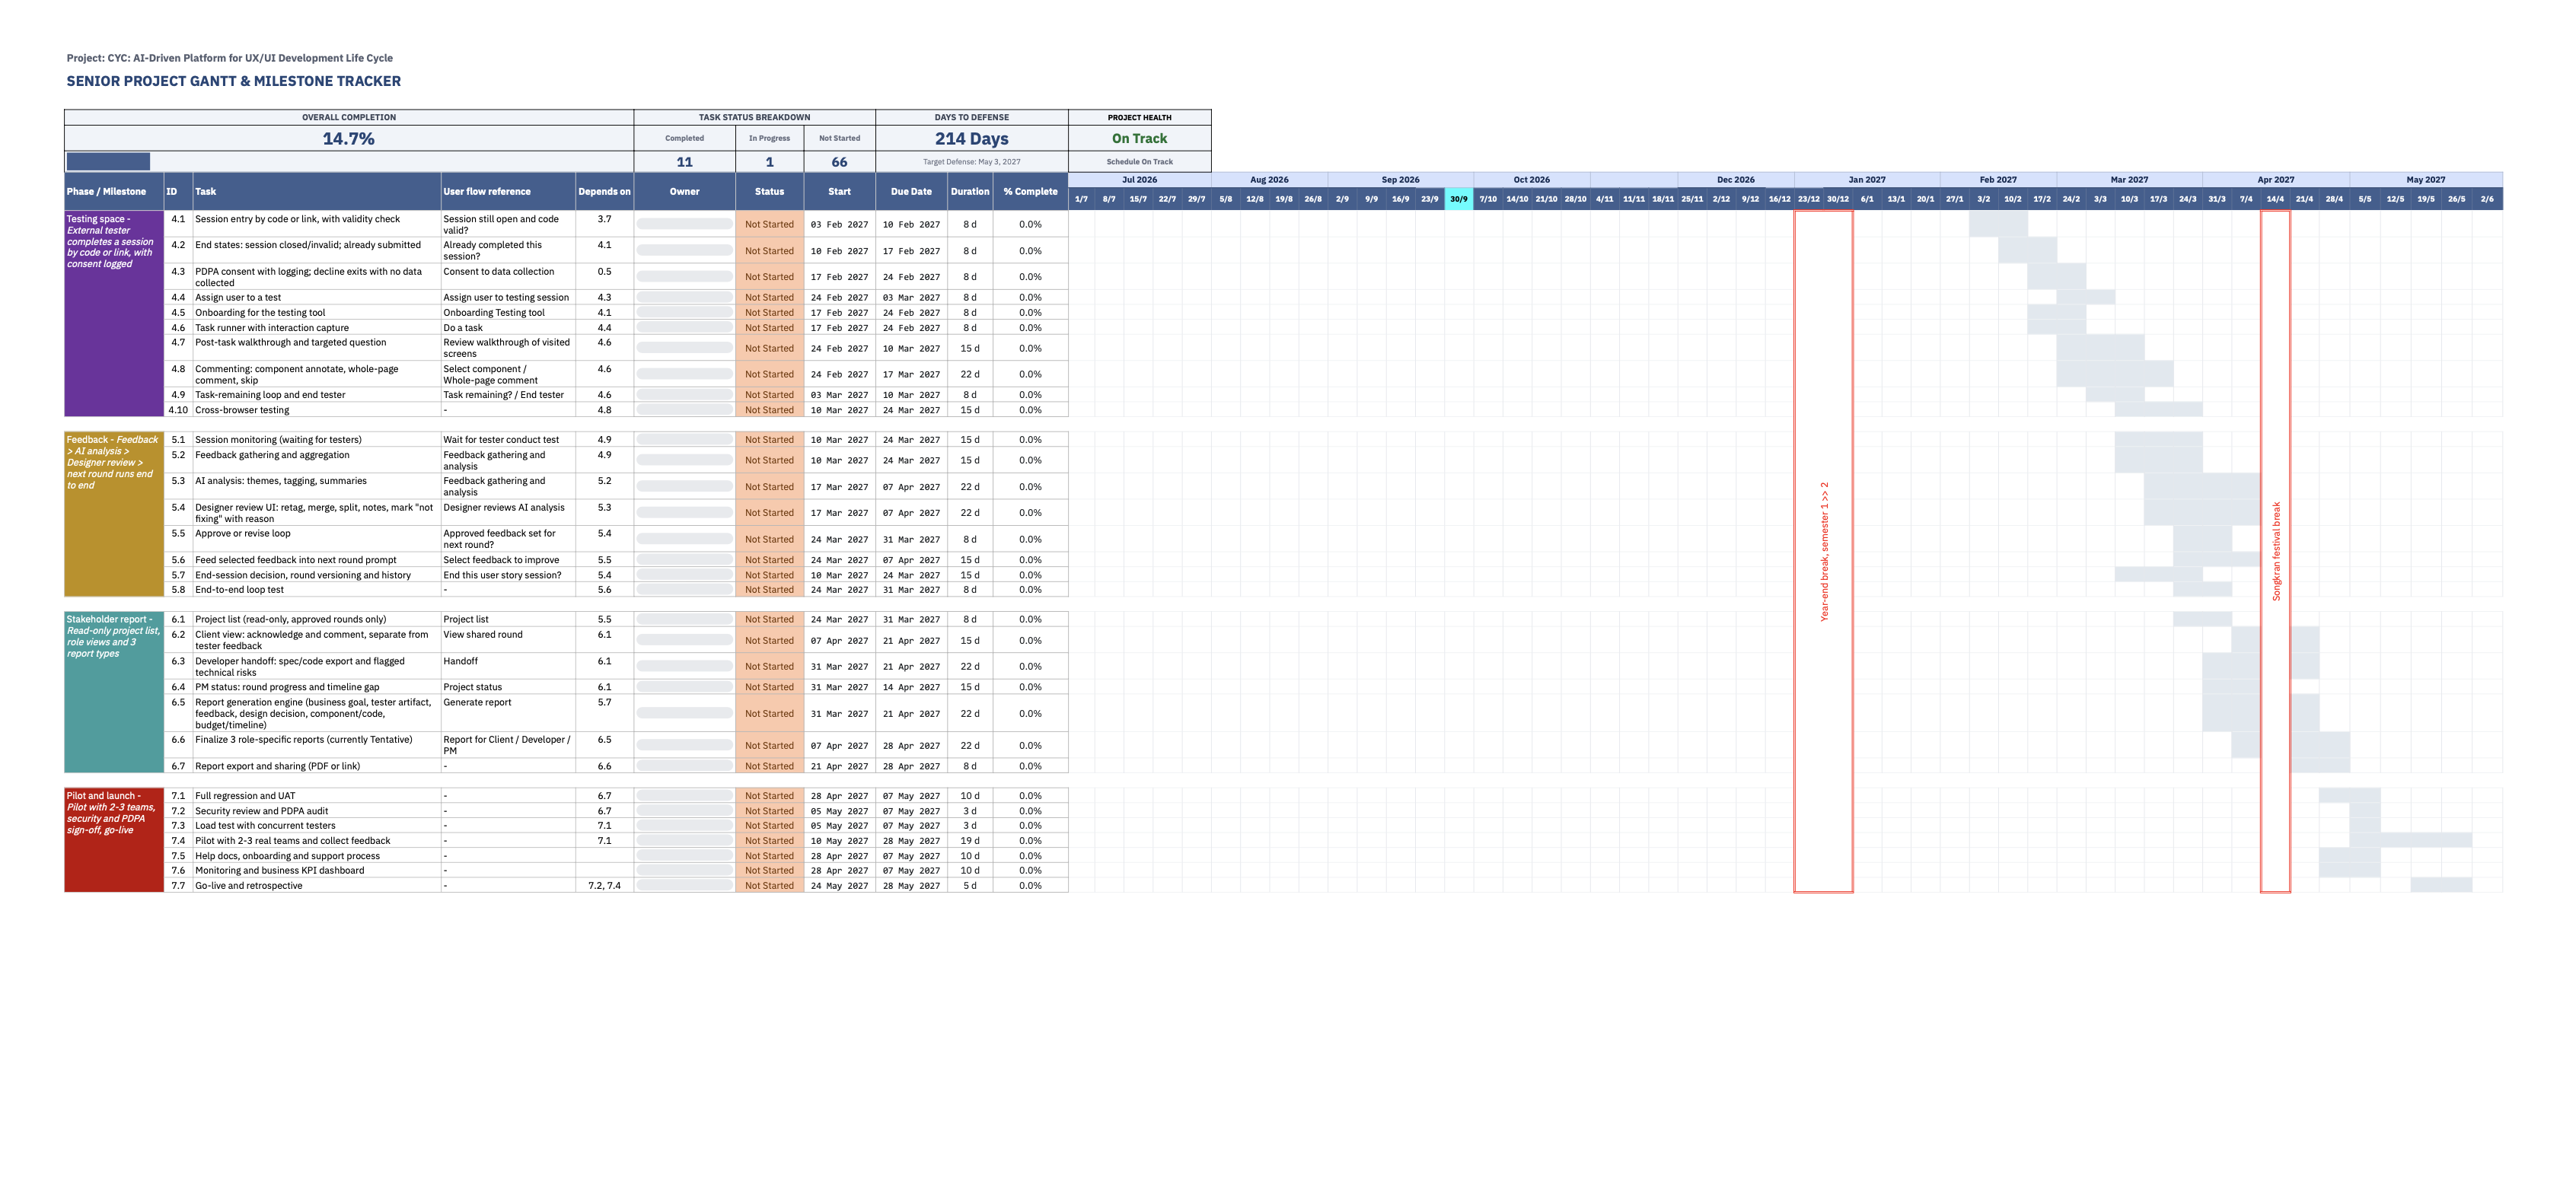
\includegraphics[
    width=0.9\textheight,
    height=0.95\linewidth,
    keepaspectratio,
    angle=90,
    origin=c
  ]{figure/gantt-sem2.png}
  \caption{Project Gantt chart สำหรับภาคการศึกษาที่ 2}
  \label{fig:gantt-semester-2}
\end{figure}
\subsection{สิ่งที่ส่งมอบ}
\subsubsection{ภาคการศึกษาที่ 1}
\begin{enumerate}
  \item \textbf{M0: Foundation}
  \begin{itemize}
    \item Software Requirement Specification, Data Model, System Architecture, Design System \& UI Kit, PDPA \& Consent, CI/CD, Sprint planning
  \end{itemize}
  \item \textbf{M1: Secure Access}
  \begin{itemize}
    \item ระบบสามารถสมัครสมาชิกพร้อมยืนยันอีเมล, เข้าสู่ระบบ, ลืมและรีเซ็ตรหัสผ่าน, ระบบสิทธิ์ตามบทบาท (Designer, Client, Developer, PM)
  \end{itemize}
  \item \textbf{M2: Project Setup}
  \begin{itemize}
    \item ระบบสามารถสร้าง organization และโปรเจกต์, แบบฟอร์ม Design Intent (description, persona, design guideline, CI, tone of voice)
  \end{itemize}
  \item \textbf{M3: AI Design Generation}
  \begin{itemize}
    \item ระบบสามารถสร้าง user story และ problem statement, สร้าง multi-variant UI ด้วย Generative AI, Chat-based UI refinement, prototype preview, อนุมัติและมอบหมายงานทดสอบ, สร้าง test session (โดยสามารถเข้าถึงด้วยรหัสหรือลิงก์)
  \end{itemize}
\end{enumerate}

\subsubsection{ภาคการศึกษาที่ 2}
\begin{enumerate}
  \item \textbf{M4: Testing Space}
  \begin{itemize}
    \item ผู้เข้าร่วมทดสอบสามารถเข้า session ด้วยรหัสหรือลิงก์, ทำ task พร้อมให้ข้อเสนอแนะเชิงบริบท
  \end{itemize}
  \item \textbf{M5: Feedback}
  \begin{itemize}
    \item ระบบสามารถรวบรวมข้อเสนอแนะ,ปัญญาประดิษฐ์สามารถวิเคราะห์รูปแบบ ข้อมูลเชิงลึก และประเด็นสำคัญ, Designer ตรวจทานและแก้ไขผลการวิเคราะห์, เลือกข้อเสนอแนะที่จะปรับปรุงในรอบถัดไป, บันทึกประวัติแต่ละรอบ
  \end{itemize}
  \item \textbf{M6: Stakeholder Report}
  \begin{itemize}
    \item ระบบสามารถแสดงหน้ารายการโปรเจกต์ (อ่านอย่างเดียว), มุมมองของ Client, Developer และ PM, รายงานสำหรับแต่ละบทบาท พร้อมส่งออก PDF หรือลิงก์
  \end{itemize}
  \item \textbf{M7: Pilot and Launch}
  \begin{itemize}
    \item ทดสอบระบบ (UAT, Load test, Security Test), ทดลองใช้กับ 2–3 ทีมตัวอย่าง, เอกสารการประกอบการใช้งาน, เปิดใช้งานจริง
  \end{itemize}
\end{enumerate}


\chapter{ทฤษฎีความรู้และงานที่เกี่ยวข้อง}
\thaijustify{
  ในบทที่ 2 นี้จะกล่าวถึงทฤษฎีที่เกี่ยวข้องที่ใช้ในการทำงานและการศึกษาเพื่อบรรลุวัตถุประสงค์ อธิบายคำศัพท์หรือภาษาทาง
คอมพิวเตอร์ เทคโนโลยีที่จะนำมาประยุกต์ใช้งานและแก้ปัญหาต่าง ๆ ในโครงงาน รวมไปถึงงานวิจัย ผลิดภัณฑ์ หรือโครง
งานที่นำมาใช้อ้างอิง เพื่อนำมาสังเคราะห์เป็นกรอบแนวคิดในการแก้ปัญหาและกำหนดขอบเขตของโครงงาน
}

\section{ทฤษฎีที่เกี่ยวข้อง}

\subsection{UX/UI Development Life Cycle: UX/UI DLC}
\thaijustify{
  กระบวนการออกแบบประสบการณ์ผู้ใช้และส่วนต่อประสานผู้ใช้เป็นกระบวนการที่เน้นผู้ใช้เป็นศูนย์กลางและต้องอาศัยการทำซ้ำอย่างต่อเนื่อง (Iterative process) โดยทั่วไปนักออกแบบจะต้องผ่านขั้นตอนตั้งแต่การรวบรวมความต้องการ การทำความเข้าใจผู้ใช้ (Empathize) การระบุปัญหา (Define) การระดมความคิด (Ideate) การสร้างต้นแบบ (Prototype) และการทดสอบ (Test)
} 
\thaijustify{อย่างไรก็ตาม ในทางปฏิบัติกระบวนการเหล่านี้นักออกแบบมักเผชิญข้อจำกัดด้านเวลา ประสบการณ์ และทรัพยากร เนื่องจากการสร้างโครงร่างหน้าจอ (Wireframes) และต้นแบบ (Prototypes) ส่วนใหญ่มักต้องสร้างด้วยมือ ซึ่งเป็นกระบวนการที่ใช้เวลาและแรงงานสูง (Labor-intensive) \cite{suh2025storyensemble} ส่งผลให้ทีมนักออกแบบมีเวลาเหลือไม่เพียงพอในการทดสอบดีไซน์กับผู้ใช้จริงก่อนถึงกำหนดส่งมอบงาน บ่อยครั้งทีมนักออกแบบจึงต้องลดจำนวนผู้ทดสอบ ข้ามขั้นตอนการทดสอบ หรือไม่สามารถนำข้อเสนอแนะที่ได้ไปปรับปรุงแก้ไขได้ทันเวลา ทำให้การตัดสินใจออกแบบถูกผลักดันด้วยความกดดันด้านเวลามากกว่าข้อมูลเชิงลึกที่ผ่านการตรวจสอบแล้วซึ่งการนำปัญญาประดิษฐ์เข้ามาช่วยสร้างต้นแบบจะสามารถลดระยะเวลาในแต่ละรอบการออกแบบและช่วยให้การทดสอบทำได้บ่อยขึ้น \cite{feng2023designing, yuan2024towards}
}

\subsection{ระเบียบวิธีการทดสอบการใช้งาน (Usability test)}
\thaijustify{
  การทดสอบกับผู้ใช้เป็นหัวใจสำคัญในการหาข้อบกพร่องและข้อควรปรับปรุงของงานออกแบบ โดยงานวิจัยชี้ให้เห็นว่าการทดสอบบ่อยครั้งกับกลุ่มตัวอย่างขนาดเล็ก ให้ข้อมูลเชิงลึกที่นำไปปรับปรุงได้จริงมากกว่าการทดสอบสเกลใหญ่แต่นาน ๆ ครั้ง \cite{nielsen2000five} สอดคล้องกับผลการศึกษาที่พบว่าปัญหาด้านการใช้งานส่วนใหญ่ถูกค้นพบได้ตั้งแต่ผู้เข้าร่วมทดสอบกลุ่มแรก ๆ และผู้ใช้ที่เพิ่มขึ้นให้ข้อมูลใหม่น้อยลงเรื่อย ๆ \cite{virzi1992refining, nielsen1993mathematical} ในวงจรการพัฒนามีระเบียบวิธีทดสอบการใช้งานที่นิยมใช้ ดังนี้
  \begin{itemize}
      \item \textbf{Usability Test} เป็นการทดสอบเพื่อให้ผู้เข้าร่วมทดสอบลองใช้งานระบบและหาจุดที่ใช้งานยากหรือติดขัด ซึ่งในขณะที่ทำการทดสอบผู้เข้าร่วมทดสอบจำเป็นต้องคิดไปด้วยพูดไปด้วย (Thinking-Aloud)โดยนักออกแบบจะคอยสังเกตพฤติกรรมและรับฟังความคิดเห็นของผู้เข้าร่วมทดสอบขณะทำภารกิจที่กำหนด \cite{rubin2008handbook, dumas1999practical, nielsen1993usability}
      \item \textbf{A/B Test} เป็นกระบวนการนำเสนอทางเลือกการออกแบบ (Variants) ที่แตกต่างกันให้กับผู้ใช้ เพื่อเปรียบเทียบประสิทธิภาพการใช้งานและรวบรวมข้อเสนอแนะก่อนที่จะตัดสินใจออกแบบในขั้นตอนถัดไป ในภาคอุตสาหกรรม A/B Test มักหมายถึงการทดลองแบบควบคุมบนระบบจริง (Online Controlled Experiment) ที่วัดผลด้วยสถิติจากผู้ใช้จำนวนมาก \cite{kohavi2009controlled, kohavi2020trustworthy} อย่างไรก็ตาม วิธีนี้ให้ผลเป็นตัวเลขว่าทางเลือกใดทำงานได้ดีกว่า แต่ไม่อธิบายเหตุผลเบื้องหลังพฤติกรรมของผู้ใช้ จึงควรใช้ร่วมกับการรวบรวมข้อมูลเชิงคุณภาพ \cite{nielsen2005abtesting} ในโครงงานนี้ A/B Test หมายถึงการให้ผู้ใช้กลุ่มเล็กลองใช้ต้นแบบสองรูปแบบและให้ข้อเสนอแนะในรอบการทดสอบ ซึ่งเป็นแนวทางเชิงคุณภาพ
      \item \textbf{Comparative Usability Test} มีหลักการคล้าย A/B Test แต่อาจเน้นการประเมินเชิงคุณภาพและให้ผู้ใช้เปรียบเทียบความพึงพอใจระหว่างดีไซน์ 2-5 รูปแบบ งานวิจัยพบว่าการให้ผู้ใช้เห็นทางเลือกการออกแบบหลายแบบพร้อมกัน ช่วยให้ผู้ใช้ให้ข้อวิจารณ์ได้เปิดกว้างและลึกกว่าการประเมินดีไซน์เดียว \cite{tohidi2006getting} อีกทั้งการสร้างต้นแบบหลายแบบยังนำไปสู่ผลงานที่ดีขึ้นและมีความหลากหลายของแนวคิดมากขึ้น \cite{dow2010parallel}
  \end{itemize}
  ความท้าทายหลักของการทำ A/B Test หรือทดสอบเชิงเปรียบเทียบซ้ำ ๆ คือภาระงานที่สูง เนื่องจากนักออกแบบต้องเตรียม multi-variant UI รวบรวมและจัดระเบียบข้อเสนอแนะของผู้ใช้ ตลอดจนตีความผลลัพธ์ก่อนเริ่มวงจรการทำซ้ำรอบใหม่ด้วยตนเอง โครงงานนี้จึงถูกพัฒนาขึ้นเพื่อประยุกต์ใช้ Generative AI เข้าสู่กระบวนการ A/B Testing ให้ผู้ใช้สามารถให้ข้อเสนอแนะลงบนต้นแบบโดยตรง และลดภาระของนักออกแบบในการวิเคราะห์ข้อมูลจำนวนมาก
}

\subsection{การค้นหาหรือสกัดความต้องการด้วยการใช้ต้นแบบ}
\thaijustify{
  การสกัดความต้องการของผู้ใช้เป็นขั้นตอนที่สำคัญในการพัฒนาระบบ จากการศึกษาของ Pacheco et al. \cite{pacheco2018} พบว่าการสร้างต้นแบบเป็นหนึ่งในเทคนิคการสกัดความต้องการที่มีความสมบูรณ์และเป็นที่ยอมรับ นอกจากนี้ Kolthoff et al. \cite{kolthoff2024} ยังระบุว่าการใช้ High-fidelity UI prototype ช่วยให้สามารถรวบรวมข้อเสนอแนะที่เฉพาะเจาะจงได้ดียิ่งขึ้น การทดสอบการใช้งานด้วยต้นแบบก่อนการพัฒนาจริงยังช่วยหลีกเลี่ยงข้อจำกัดของการทดสอบบนระบบจริง เช่น A/B Testing บนหน้าเว็บจริง ซึ่ง Lu et al. \cite{lu2026} พบว่ามักมีปัญหาจากปริมาณผู้ใช้ (Traffic) ที่หายาก ระยะเวลาการทดสอบที่ยาวนาน และต้นทุนที่สูง
}

\subsection{ความสัมพันธ์ระหว่างความชอบของผู้ใช้และประสิทธิภาพการใช้งาน}
\thaijustify{
  ในการทดสอบการใช้งาน ความชอบของผู้ใช้อาจไม่ได้สะท้อนถึงประสิทธิภาพเสมอไป ข้อมูลจาก Nielsen Norman Group \cite{nngroup_satisfaction} ระบุว่าความชอบของผู้ใช้สอดคล้องกับตัวชี้วัดด้านประสิทธิภาพการใช้งาน (Usability metrics) ในระดับสูงสุดเพียงร้อยละ 70 ของเวลาทั้งหมด นอกจากนี้ การใช้ตัวเลขจากการทดสอบเชิงคุณภาพในกลุ่มตัวอย่างขนาดเล็กอาจทำให้เกิดความเข้าใจผิดได้ \cite{nngroup_qualitative} ดังนั้น โครงงาน CYC จึงตัดสินใจออกแบบระบบให้ตีความผลการโหวตและข้อเสนอแนะเป็นข้อมูลเชิงคุณภาพเพื่อค้นหาความต้องการเท่านั้น โดยไม่นำไปใช้เป็นหลักฐานวัดประสิทธิภาพเชิงพฤติกรรม เช่น เวลาที่ใช้ (Time-on-task) อัตราการคลิก (Click-through-rate: CTR) หรืออัตราการแปลง (Conversion rate: CVR)
}

\subsection{ทฤษฎีผู้มีส่วนได้ส่วนเสียและการถ่วงน้ำหนัก}
\thaijustify{
  ข้อเสนอแนะที่ได้จากผู้มีส่วนได้ส่วนเสียมักปะปนกันระหว่างปัญหาการใช้งานจริง (Pain point) กับความชอบส่วนตัวของบุคคลนั้น ๆ Shukla et al. \cite{shukla2025} พบว่าผู้มีส่วนได้ส่วนเสียบางรายมักใช้อำนาจตำแหน่งกำหนดทิศทางงาน ทำให้ความต้องการเปลี่ยนไปตามการเมืองภายในองค์กรมากกว่าข้อมูลของผู้ใช้จริง สอดคล้องกับแนวคิดของ Mitchell et al. \cite{mitchell1997} ที่เสนอว่าความสำคัญของผู้มีส่วนได้ส่วนเสียขึ้นอยู่กับปัจจัยด้านอำนาจ ความชอบธรรม และความเร่งด่วน โครงงานนี้จึงนำทฤษฎีนี้มาประยุกต์ใช้โดยกำหนดบทบาทและน้ำหนักการตัดสินใจที่แตกต่างกันระหว่างนักออกแบบ ผู้เข้าร่วมทดสอบ และผู้มีส่วนได้ส่วนเสีย พร้อมทั้งแสดงผลลัพธ์แยกตามกลุ่มเพื่อลดอคติเชิงอำนาจในการตัดสินใจ
}

\subsection{ข้อกำหนดระบบการออกแบบด้วย Generative AI}
\thaijustify{
  การทำงานกับ Generative AI เพื่อ multi-variant UI จำเป็นต้องมีกรอบควบคุม (Guardrails) เพื่อให้ผลลัพธ์ที่ได้สอดคล้องกับอัตลักษณ์ของผู้ว่าจ้างหรือผลิตภัณฑ์นั้น ๆ Figma \cite{figma_agent} ระบุว่าการใช้ Variables และ Design Tokens ช่วยเป็นกรอบให้ Generative AI สามารถสร้างทางเลือกการออกแบบที่ถูกต้องได้ และ Design Tokens Community Group \cite{designtokens2025} ได้กำหนดมาตรฐานรูปแบบไฟล์สำหรับการแลกเปลี่ยน Design tokens ระหว่างเครื่องมือไว้ โครงงานนี้จึงกำหนดให้ Color tokens และ Design system เป็นข้อบังคับใช้ควบคุมในการสร้าง UI ด้วย Generative AI และใช้ตรวจสอบความถูกต้องก่อนการส่งมอบ
}
% /2.1.6 - 2.2.3 เอามารวมกันเลย
\section{โครงงาน งานวิจัยหรือผลิตภัณฑ์ที่เกี่ยวข้อง}

\subsection{การสร้าง UI และการสกัดความต้องการด้วย Generative AI}
\thaijustify{
  การใช้แบบจำลองภาษาขนาดใหญ่ (LLMs) ในการสร้าง UI ยังคงมีความท้าทาย Kolthoff et al. \cite{kolthoff2024} ประเมินการสร้าง HTML/CSS ด้วย GPT-4o และพบข้อบกพร่อง 3 กลุ่มหลัก ได้แก่ การจัดวาง (Layout) ฟังก์ชันที่ตีความผิด และสไตล์ที่ไม่สอดคล้องกัน ในขณะที่ Ataei et al. \cite{ataei2025} ใช้ LLM Agents จำลองเป็นผู้ใช้เพื่อสกัดความต้องการแฝง แต๋โครงงานนี้เลือกใช้ผู้ทดสอบที่เป็นมนุษย์จริงแทนการจำลองผู้ใช้ นอกจากนี้ Suh et al. \cite{suh2024} ได้เสนอแนวทางการให้ LLM สร้างแบบร่างของงานขึ้นมาก่อนสร้างคำตอบ ซึ่งเป็นแนวคิดที่โครงงานนี้อาจนำมาใช้สร้างทางเลือกการออกแบบ 2 รูปแบบที่แตกต่างกัน
}
% อาจจะรวม 2.2.1 ไปกับ 2.2.2 ไปเลยก็ได้
\subsection{การวิเคราะห์ข้อเสนอแนะ และอคติของปัญญาประดิษฐ์}
\thaijustify{
  การใช้ LLM ในการวิเคราะห์ข้อมูลเชิงคุณภาพ เช่น CollabCoder \cite{gao2024} ที่ให้ AI ช่วยเสนอโค้ดในขั้นตอน Open coding หรือ PaTAT \cite{gebreegziabher2023} ที่เรียนรู้รูปแบบการเข้ารหัสเชิงคุณภาพ อย่างไรก็ตาม LLM มักมีอคติเชิงลบ (Negative bias) ในงานที่ต้องตัดสินใจแบบ Yes-No \cite{song2025} และมีข้อจำกัดในการดึงลักษณะสำคัญของข้อมูลเพื่อสร้าง Persona หากปราศจากการชี้แนะจากมนุษย์ \cite{shin2024} โครงงานจึงกำหนดให้มนุษย์เข้ามามีส่วนร่วมในการตัดสินใจร่วมกับปัญญาประดิษฐ์ ในกระบวนการจำแนกข้อเสนอแนะระหว่าง Pain point กับ ความชอบส่วนตัว
}

\subsection{แนวทางการปฏิสัมพันธ์ระหว่างมนุษย์กับปัญญาประดิษฐ์}
\thaijustify{
  Amershi et al. \cite{amershi2019} เสนอแนวทางสำหรับการปฏิสัมพันธ์ระหว่างมนุษย์กับปัญญาประดิษฐ์ เช่น การให้ระบบบอกความสามารถของตนเอง การอนุญาตให้แก้ไขผลลัพธ์ได้ง่าย และการอธิบายเหตุผลของการกระทำ Pourasad \& Maalej \cite{pourasad2025} พบว่า UX-LLM ที่ใช้ทำนายปัญหาการใช้งานในแอปพลิเคชันยังมีค่า Recall ต่ำและพลาดปัญหาสำคัญส่วนใหญ่ การทดสอบด้วย AI จึงเป็นเพียงส่วนเสริม ไม่สามารถทดแทนผู้ใช้จริงได้ โครงงานนี้จึงออกแบบให้ผู้ใช้จริงเป็นผู้ให้ความเห็น ส่วนปัญญาประดิษฐ์ทำหน้าที่วิเคราะห์เบื้องต้นเท่านั้นแล้วจึงให้มนุษย์ตัดสินใจในขั้นตอนสุดท้าย
}

\subsection{ผลิตภัณฑ์และเครื่องมือในตลาดปัจจุบัน}
\thaijustify{
  จากการสำรวจผลิตภัณฑ์ที่เกี่ยวข้อง ณ ปัจจุบัน พบว่าเครื่องมือแต่ละกลุ่มมีจุดเด่นและข้อจำกัดที่ต่างกัน ได้แก่
  \begin{itemize}
    \item \textbf{เครื่องมือ A/B Testing (เช่น Kameleoon, Otter)} มักทำงานกับเว็บไซต์ที่พัฒนาเสร็จแล้ว (Live site) เพื่อวัดพฤติกรรมผู้ใช้ ซึ่งต่างจากโครงงานนี้ที่ทำงานกับต้นแบบก่อนการพัฒนา \cite{kameleoon, otterab}
    \item \textbf{เครื่องมือทดสอบผู้ใช้ก่อนเขียนโค้ด (เช่น Lyssna, Useberry)} มีฟังก์ชัน Preference testing สำหรับเปรียบเทียบดีไซน์คู่กัน แต่ยังไม่มีการใช้ AI สร้างทางเลือก (Variants) หรือใช้ AI แยกแยะ Pain point ออกจากความชอบในระบบเดียวกัน \cite{lyssna, useberry}
    \item \textbf{เครื่องมือออกแบบที่มีปัญญาประดิษฐ์เป็นตัวช่วยในการทำงาน (เช่น Figma Make, Figma Agent):} สามารถสร้างต้นแบบหรือ variants จากคำสั่งได้ แต่ยังไม่มีระบบรวบรวมข้อเสนอแนะจากผู้ทดสอบหลายกลุ่มเพื่อนำมาวิเคราะห์ร่วมกัน \cite{figma_agent}
    \item \textbf{เครื่องมือตรวจงานด้วยหมุดคอมเมนต์ (เช่น BugHerd, Marker.io)} ให้ผู้ใช้ปักหมุดพร้อมแนบข้อมูลทางเทคนิคได้ แต่ยังขาดฟังก์ชันการเปรียบเทียบ 2 ทางเลือกพร้อมการโหวต และการจำแนกข้อเสนอแนะด้วยปัญญาประดิษฐ์ \cite{bugherd, markerio}
  \end{itemize}
}

\section{ภาษาคอมพิวเตอร์เเละเทคโนโลยี}

\subsection{แบบจำลองภาษาขนาดใหญ่ (Large Language Models: LLM)}
\thaijustify{
  โครงงานใช้ LLM (เช่น muse-glimmer-30b) เป็นเทคโนโลยีหลักในการประมวลผลคำสั่ง (Prompt) เพื่อสร้าง multi-variant UI รวมถึงใช้ในการวิเคราะห์ภาษาธรรมชาติ (Natural Language Processing) เพื่อจำแนกประเภทของข้อเสนอแนะ สรุปผล และสร้าง Persona Artifact จากข้อมูลผู้เข้าร่วมทดสอบ
}

\subsection{เทคโนโลยีการสร้างส่วนติดต่อผู้ใช้ (HTML/CSS \& Design System)}
\thaijustify{
  ต้นแบบที่ระบบสร้างขึ้นจะอยู่ในรูปแบบของ HTML/CSS ที่มีความละเอียดสูง (High-fidelity) เพื่อให้ผู้ทดสอบสามารถคลิก ใช้งาน และให้ข้อเสนอแนะเชิงบริบทได้อย่างสมจริง โดยจะมีการควบคุมคุณภาพของโค้ดที่สร้างด้วยปัญญาประดิษฐ์ผ่านการใช้ Design Tokens ที่กำหนดไว้ล่วงหน้า
}

\section{สรุปการศึกษาค้นคว้า}
\thaijustify{
  งานวิจัยที่ผ่านมาชี้ให้เห็นว่า Generative AI สามารถช่วยลดภาระของนักออกแบบในกระบวนการ UX/UI ที่มักถูกจำกัดด้วยเวลาและแรงงานในการสร้าง wireframe และ prototype ด้วยมือ \cite{suh2025storyensemble, feng2023designing, yuan2024towards} โดยเฉพาะในขั้นตอนการทดสอบการใช้งานที่งานวิจัยยืนยันว่าการทดสอบบ่อยครั้งกับกลุ่มตัวอย่างขนาดเล็กให้ข้อมูลเชิงลึกที่มีประโยชน์มากกว่าการทดสอบสเกลใหญ่แต่นาน ๆ ครั้ง \cite{nielsen2000five, virzi1992refining, nielsen1993mathematical} และการใช้ต้นแบบความละเอียดสูง (high-fidelity prototype) ยังช่วยสกัดความต้องการของผู้ใช้ได้ดีกว่าการทดสอบบนระบบจริงซึ่งมีข้อจำกัดด้าน traffic และต้นทุน \cite{pacheco2018, kolthoff2024, lu2026} อย่างไรก็ตาม ความชอบของผู้ใช้ไม่ได้สะท้อนประสิทธิภาพการใช้งานเสมอไป \cite{nngroup_satisfaction, nngroup_qualitative} และข้อเสนอแนะจากผู้มีส่วนได้ส่วนเสียมักปะปนระหว่าง pain point กับความชอบส่วนตัวหรืออำนาจทางการเมืองภายในองค์กร จึงจำเป็นต้องมีการถ่วงน้ำหนักตามทฤษฎีผู้มีส่วนได้ส่วนเสีย \cite{shukla2025, mitchell1997} นอกจากนี้ การนำ LLM มาสร้าง UI และวิเคราะห์ข้อเสนอแนะเชิงคุณภาพยังพบข้อจำกัดสำคัญ เช่น ปัญหาด้าน layout และฟังก์ชันที่ตีความผิด \cite{kolthoff2024} อคติเชิงลบในการตัดสินใจแบบ yes-no \cite{song2025} และความสามารถในการดึงลักษณะสำคัญเพื่อสร้าง persona ที่ยังต้องอาศัยการชี้แนะจากมนุษย์ \cite{shin2024} ทำให้แนวทางที่เหมาะสมคือการออกแบบปฏิสัมพันธ์ระหว่างมนุษย์กับปัญญาประดิษฐ์ตามหลักการที่ให้ระบบอธิบายความสามารถและเหตุผลของตนได้ \cite{amershi2019} พร้อมให้มนุษย์เป็นผู้ตัดสินใจขั้นสุดท้ายแทนการพึ่งพาปัญญาประดิษฐ์ทั้งหมด \cite{pourasad2025} ขณะที่การสำรวจผลิตภัณฑ์ที่มีอยู่แล้วในตลาด เช่น เครื่องมือ A/B testing บนเว็บไซต์จริง \cite{kameleoon, otterab} เครื่องมือทดสอบก่อนเขียนโค้ด \cite{lyssna, useberry} เครื่องมือออกแบบที่มีปัญญาประดิษฐ์ช่วยสร้าง variant \cite{figma_agent} และเครื่องมือปักหมุดคอมเมนต์ \cite{bugherd, markerio} ท้ังหมดยังคงมีช่องว่างร่วมกัน คือ นักออกแบบยังไม่สามารถใช้ปัญญาประดิษฐ์ช่วยในการทำงานทั้งกระบวนการในแพลตฟอร์มเดียวซึ่งเป็นช่องว่างที่โครงงานนี้ให้ความสำคัญ
}

% \thaijustify{
%   และจากการทบทวนวรรณกรรมทำให้เห็นช่องว่างทางการวิจัย คือ ปัจจุบันยังไม่มีเครื่องมือหรืองานวิจัยใดที่รวบรวมความสามารถทั้ง 4 ด้านไว้ในระบบเดียว ได้แก่ (1) การใช้ปัญญาประดิษฐ์สร้าง multi-variant UI ภายใต้ Design system ที่กำหนด (2) การให้ผู้ทดสอบให้ข้อเสนอแนะ (3) การใช้ปัญญาประดิษฐ์แยกแยะ pain point ออกจากความชอบร่วมกับการตัดสินใจของนักออกแบบ และ (4) การสร้าง Persona Artifact จากผลลัพธ์ 
% }  
% \thaijustify{สิ่งที่โครงงานนี้ควรให้ความสำคัญเป็น คือ การพัฒนาแพลตฟอร์มนี้ให้ครอบคลุมกระบวนการตั้งแต่รับโจทย์ สร้างต้นแบบ รวบรวมข้อเสนอแนะ และวิเคราะห์ผลลัพธ์ เพื่อให้นักออกแบบสามารถส่งมอบงานที่มีการตรวจสอบความต้องการของผู้ใช้ที่แท้จริง พร้อมด้วย design system และต้นแบบที่ลูกค้าพึงพอใจให้นักพัฒนาต่อไปได้อย่างมีประสิทธิภาพ
% }



\chapter{วิธีการดำเนินงาน}
% \thaijustify{
%   [ภาพรวมของบทนี้]
% }
\begin{samepage}
\section{Preliminary User Flow}
\begin{figure}[H]
  \centering
  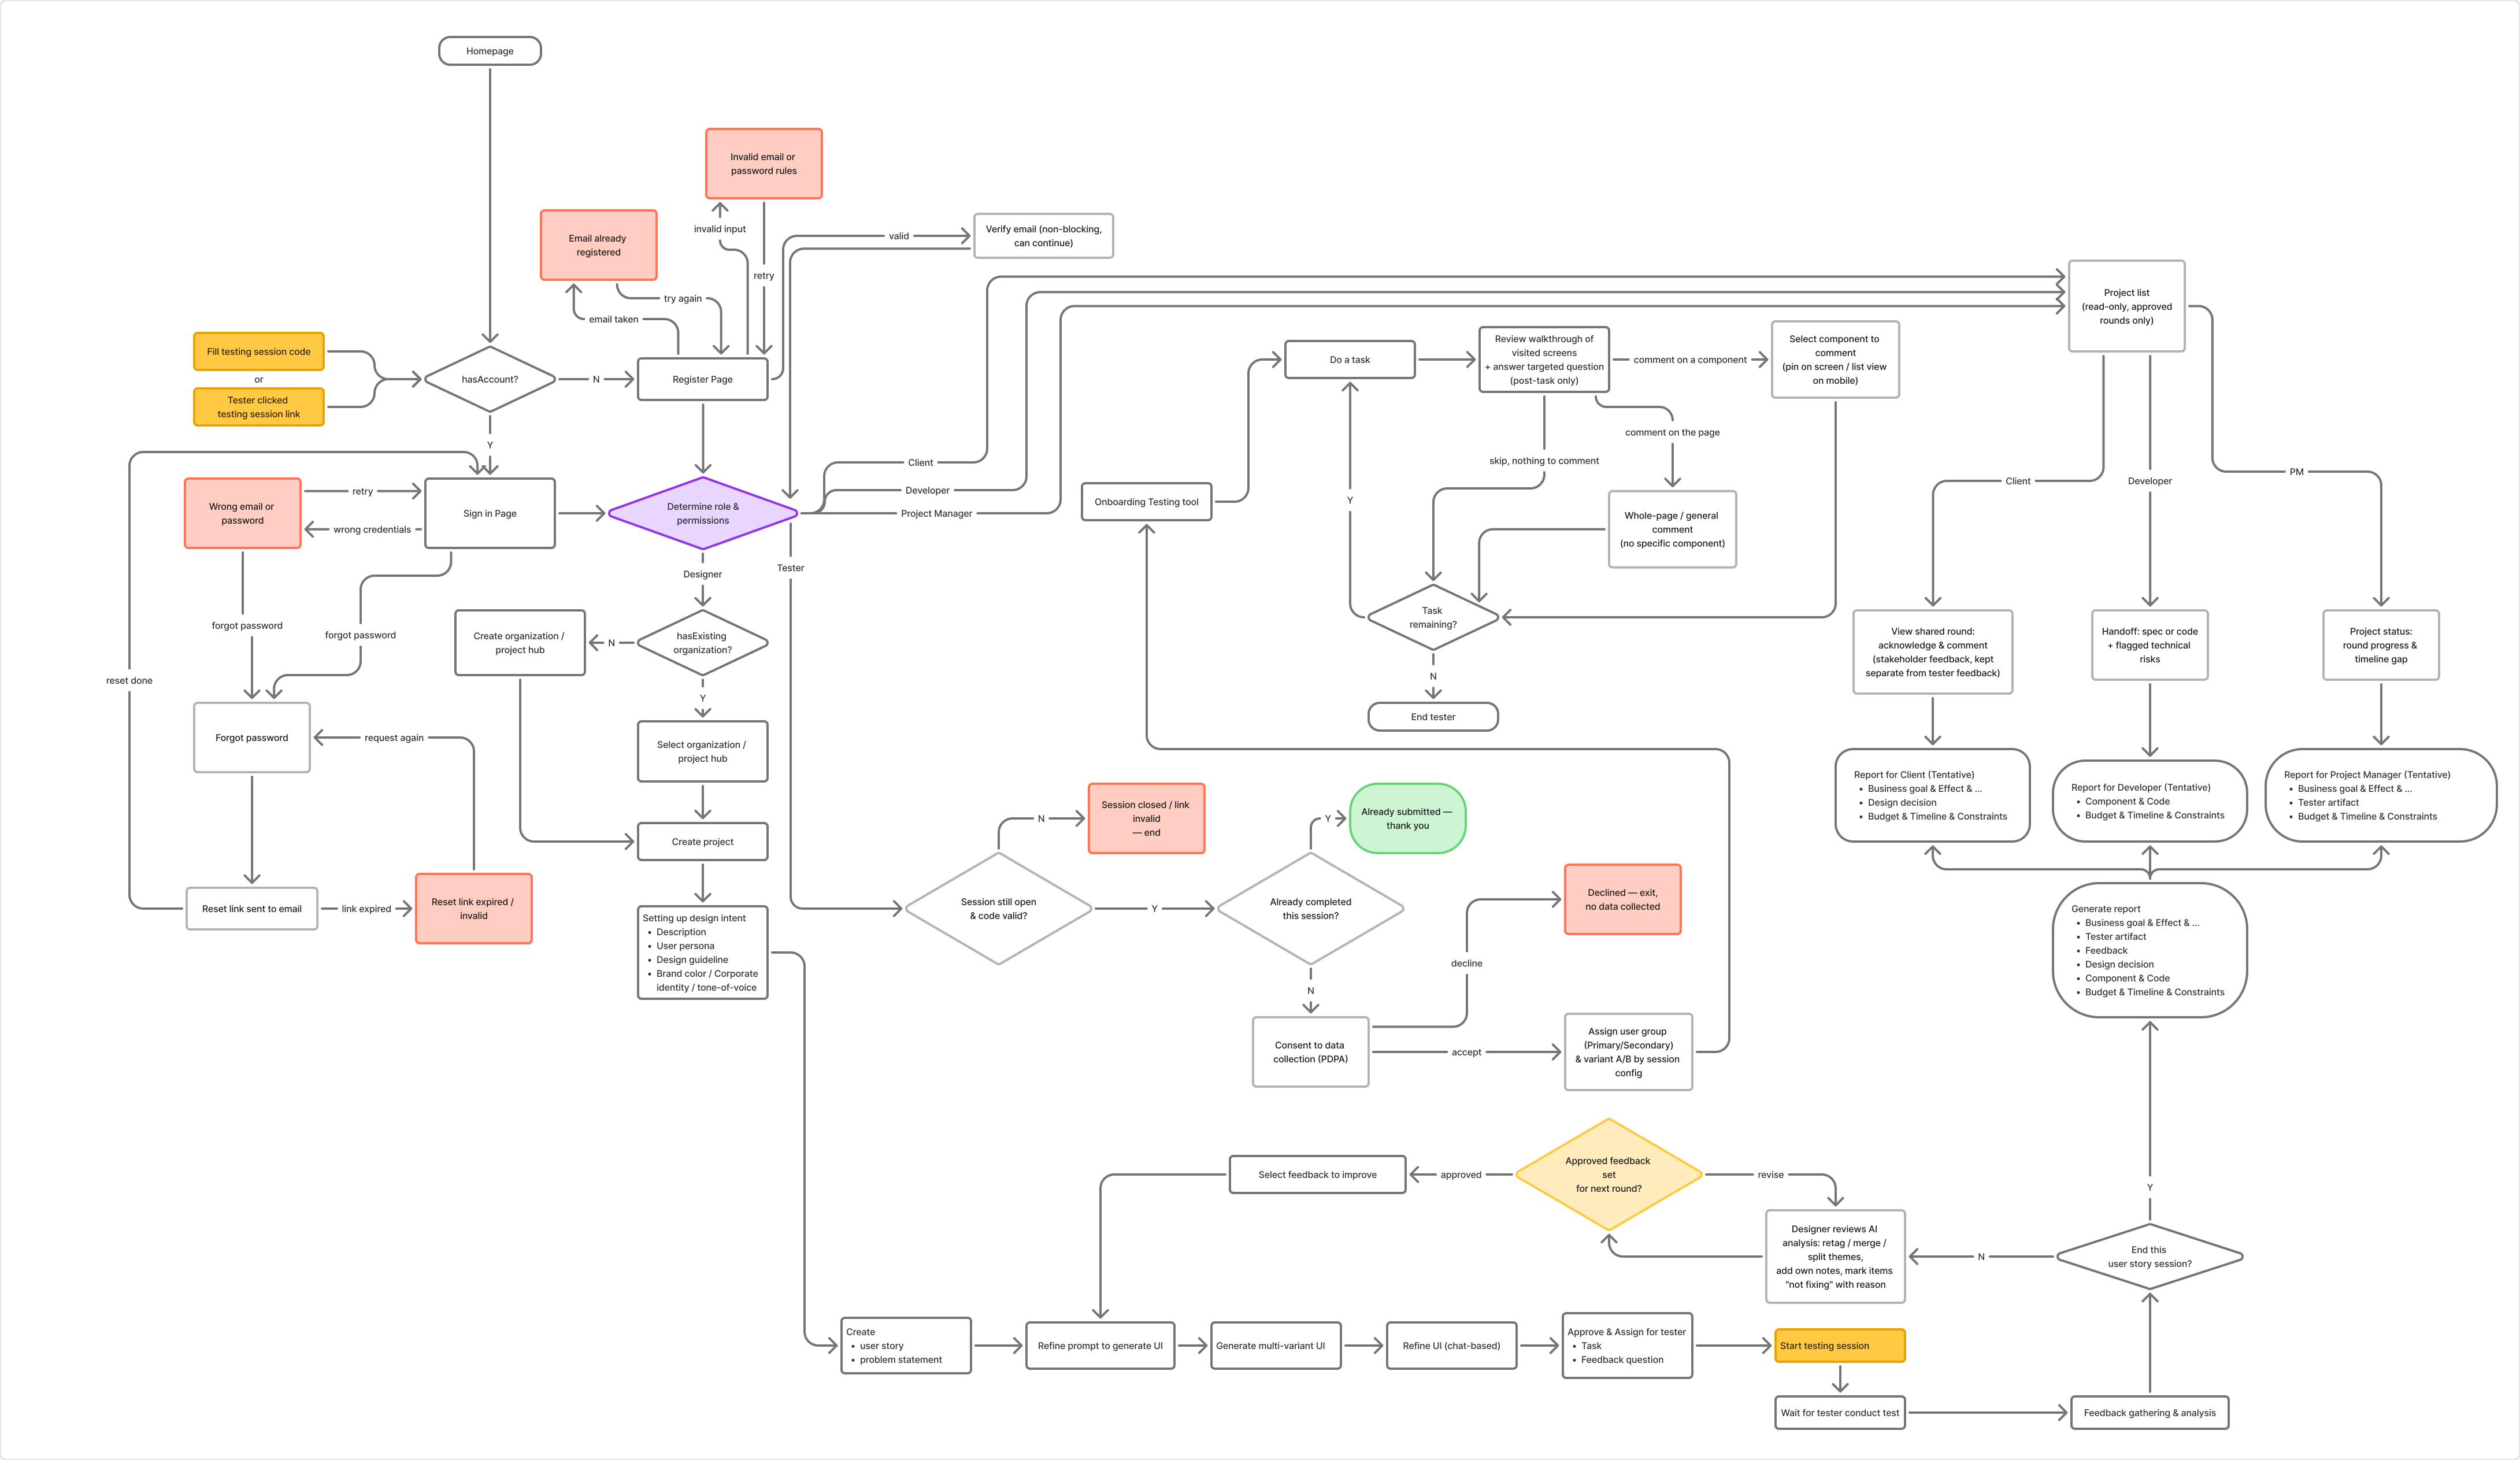
\includegraphics[
    width=0.72\textheight,
    height=0.95\linewidth,
    keepaspectratio,
    angle=90,
    origin=c
  ]{figure/cyc-user-flow.png}
  \caption{Preliminary user flow of platform}
  \label{fig:preliminary-user-flow}
\end{figure}
\end{samepage}

\section{System Architecture \& Tech Stack}
\begin{figure}[H]
  \centering
  \includegraphics[
    width=\linewidth,
    height=0.78\textheight,
    keepaspectratio
  ]{../prism-uploads/tech-stack.png}
  \caption{Tech stack and system architecture of platform}
  \label{fig:tech-stack-system-architecture}
\end{figure}

% \chapter{ผลการดำเนินงาน}
% \thaijustify{
%   [ภาพรวมของบทนี้]
% }
% \section{ผลจากการดำเนินการ}
% \thaijustify{
%   [เนื้อหาในหัวข้อนี้]
% }
% \section{ผลลัพธ์จากการทดลองเปิดใช้งานซอฟต์แวร์}
% \thaijustify{
%   [เนื้อหาในหัวข้อนี้]
% }
% \section{ผลจากแบบสำรวจความพึงพอใจของซอฟต์แวร์}
% \thaijustify{
%   [เนื้อหาในหัวข้อนี้]
% }
% \section{การอภิปรายผลจากการดำเนินการ}
% \thaijustify{
%   [เนื้อหาในหัวข้อนี้]
% }

% \chapter{บทสรุป}
% \thaijustify{
%   [ภาพรวมของบทนี้]
% }
% \section{สรุปผลโครงงาน}
% \thaijustify{
%   [เนื้อหาในหัวข้อนี้]
% }
% \section{ปัญหาที่พบและการแก้ไข}
% \thaijustify{
%   [เนื้อหาในหัวข้อนี้]
% }
% \section{ข้อเสนอแนะสำหรับการพัฒนาต่อในอนาคต}
% \thaijustify{
%   [เนื้อหาในหัวข้อนี้]
% }

%%%%%%%%%%%%%%%%%%%%%%%%% Bibliography %%%%%%%%%%%%%%%%%%%%%%%%%
%: Comment this in your report to show only references you have
%: cited. Otherwise, all the references below will be shown.
% \nocite{*}



% Use the kmutt.bst for bibtex bibliography style
% You must have cpe.bib and string.bib in the correct directory
% You may go to file .bbl to manually edit the bib items.

%: Sept, 2021 by Thanin
%: Improve url breaks to prevent unnecessary big white spaces in some cases
\makeatletter
\g@addto@macro{\UrlBreaks}{\UrlOrds}
\makeatother

%: July, 2024 by Jatetanan
%: Add biblatex for managing bibs
%: Uncomment this if you're using biblatex
\printbibliography[heading=bibintoc,title={บรรณานุกรม}]

%: Uncomment \bibliographystyle and \bibliography if you're not using biblatex

%: References style
%: Examples: \bibliographystyle{bibstyle/kmutt}
% \bibliographystyle{bib/ieee}

%: References files
%: Examples: \bibliography{example/string,example/string2,example/cpe}
% \bibliography{bib/codern}

%%%%%%%%%%%%%%%%%%%%%%%%% Appendices %%%%%%%%%%%%%%%%%%%%%%%%%%%
% \appendix{ชื่อภาคผนวก A}
% [เนื้อหาภาคผนวก A]

% \appendix{ชื่อภาคผนวก B}
% [เนื้อหาภาคผนวก B]

\end{document}
%%%%%%%%%%%%%%%%%%%%%%%%%% REPORT END %%%%%%%%%%%%%%%%%%%%%%%%%%%%%%%